\documentclass[a4paper,12pt,reqno]{article}

\usepackage{styledoc19}
\addbibresource{references.bib}

\begin{document}
    \selectlanguage{russian}
    \student{БПИ 213}{В. А. Андронов}
    \supervisor{Доцент департамента \vfill программной инженерии \vfill факультета компьютерных \vfill наук, кандидат \vfill технических наук}{О. В. Максименкова}
    \project{Веб-приложение для ведения лабораторных и вычислительных экспериментов с поддержкой онтологий\unskip}

    \VKR

    \section*{\centering Реферат}
В современном мире научные исследования становятся всё более сложными и требуют эффективных инструментов для документирования, анализа и обмена данными. Одним из таких инструментов является электронный лабораторный журнал (сокращённо ELN), который позволяет учёным структурировать данные экспериментов, обеспечивать их воспроизводимость и стандартизацию. В данной работе предлагается разработка веб-приложения, реализующего функционал ELN, основное внимание уделяется возможности привязки данных эксперимента к онтологиям (например, OM2 \cite{ontology:OM2} или ChEBI \cite{ontology:СhEBI}), что позволяет унифицировать единицы измерения и улучшить интероперабельность данных. Разработанное решение может быть использовано в научных лабораториях, исследовательских центрах и образовательных учреждениях для повышения качества документирования экспериментальных данных, но в первую очередь предназначено для РТУ МИРЭА.

Использование онтологий в научных исследованиях обосновано их способностью обеспечивать семантическую совместимость данных, что особенно важно при анализе и обмене результатами между различными лабораториями и информационными системами. Согласно работе \textit{Relations in biomedical ontologies} \cite{ontology:base1}, онтологии позволяют стандартизировать представление данных, что делает их пригодными для автоматизированной обработки. В то же время, как отмечается в работе \textit{Knowledge Graphs} \cite{ontology:base2}, применение графовых баз данных значительно упрощает управление онтологиями и их интеграцию в прикладные системы, что повышает эффективность работы с научными данными.

Работа содержит 48 страниц, 10 рисунков, 1 таблицу, 40 источников.

\textit{\textbf{Ключевые слова -- онтологически-контролируемое управление данными; электронный лабораторный журнал; управление экспериментами; онтология предметной области}}

\newpage

\section*{\centering Abstract}
In today's world, scientific research is becoming increasingly complex and requires effective tools for documenting, analyzing, and sharing data. One of these tools is the electronic laboratory journal (abbreviated as ELN), which allows scientists to structure experimental data, ensure their reproducibility and standardization. This paper proposes the development of a web application that implements the ELN functionality, focusing on the possibility of linking experimental data to ontologies (for example, OM2\cite{ontology:OM2} or ChEBI \cite{ontology:СhEBI}), which makes it possible to unify units of measurement and improve data interoperability. The developed solution can be used in scientific laboratories, research centers and educational institutions to improve the quality of documentation of experimental data, but is primarily intended for RTU MIREA.

The use of ontologies in scientific research is justified by their ability to ensure semantic compatibility of data, which is especially important when analyzing and exchanging results between different laboratories and information systems. According to the work \textit{Relations in biomedical ontologies} \cite{ontology:base1}, ontologies allow you to standardize the representation of data, which makes them suitable for automated processing. At the same time, as noted in \textit{Knowledge Graphs} \cite{ontology:base2}, the use of graph databases greatly simplifies the management of ontologies and their integration into application systems, which increases the efficiency of working with scientific data.

The work contains 48 pages, 10 diagrams, 1 tables, 40 sources.

\textit{\textbf{Keywords -- ontologically-controlled data management; electronic laboratory notebook; experiment management; domain ontology}}


    \section*{\centering Основные определения, термины и сокращения}

    \phantomsection
\addcontentsline{toc}{section}{Основные определения, термины и сокращения}

\begin{description}[style=unboxed,leftmargin=0cm]

    \item[\textbf{Валидность}] -- степень соответствия полученных данных реальности.

    \item[\textbf{Вычислительный эксперимент}] -- метод исследования, при котором математические модели и компьютерные расчёты используются для анализа сложных систем и прогнозирования их поведения.

    \item[\textbf{Домен (предметная область)}] -- область знаний, к которой относится конкретное программное обеспечение.

    \item[\textbf{Интероперабельность}] -- возможность обмена и понимания данных между разными системами на основе их смыслового значения.

    \item[\textbf{Клиент-серверная архитектура}] -- принцип проектирования ПО, согласно которому клиент запрашивает данные у сервера, который их обрабатывает и отправляет обратно.

    \item[\textbf{Лабораторный эксперимент}] -- метод научного исследования, проводимый в контролируемых условиях лаборатории для проверки гипотез, изучения свойств объектов или выявления закономерностей.

    \item[\textbf{Онтология}] -- формализованное представление знаний в определённой предметной области, включающее определения понятий, их свойства и взаимосвязи между ними. Используется в искусственном интеллекте, базах знаний и прочих областях.

    \item[\textbf{Слоистая архитектура}] -- принцип проектирования ПО, согласно которому система разделена на слои, каждый из которых выполняет свою роль.

    \item[\textbf{СУБД (Система управления базами данных)}] -- программное обеспечение для создания, управления и работы с базами данных.

    \item[\textbf{API (Application Programming Interface)}] -- интерфейс программирования приложений, набор правил и инструментов для взаимодействия между программными компонентами.

    \item[\textbf{ELN (Electronic Laboratory Notebook)}] -- электронный лабораторный журнал, который используется для ведения, хранения и управления научными записями, заменяя традиционные бумажные записи.

    \item[\textbf{JWT (JSON Web Token)}] -- компактный и безопасный способ передачи информации между сторонами в виде JSON-объекта, часто используется для аутентификации.

    \item[\textbf{ORM (Object-Relational Mapping)}] -- технология, позволяющая работать с базами данных с использованием объектно-ориентированных подходов вместо SQL-запросов.

    \item[\textbf{SPA (Single Page Application)}] -- веб-приложение, которое загружается один раз и обновляет контент без полной перезагрузки страницы, улучшая пользовательский опыт.

\end{description}

    \tableofcontents

    \anonsection{\centering Введение}

Современные научные исследования требуют систематического подхода к хранению, обработке и анализу экспериментальных данных. Традиционные методы ведения лабораторных записей, основанные на бумажных журналах или неструктурированных электронных документах, затрудняют поиск информации, совместное использование данных и уменьшают их валидность. В связи с этим все большую популярность приобретают электронные лабораторные журналы, которые позволяют организованно фиксировать результаты экспериментов и облегчать их последующую обработку.

Одной из ключевых проблем, возникающих при работе с ELN, является стандартизация данных. Исследователи могут использовать разные системы единиц измерения, а также различные обозначения одних и тех же сущностей, что затрудняет интерпретацию и сравнение данных. Решением этой проблемы является использование онтологий — формализованных моделей знаний, описывающих объекты и их взаимосвязи в определенной предметной области.

В данной работе рассматривается разработка веб-приложения, реализующего концепцию ELN с возможностью привязки экспериментальных данных к онтологиям. Это позволит не только систематизировать данные, но и повысить их интероперабельность, а также упростить интеграцию с другими научными ресурсами. В качестве онтологических источников предлагается использование стандартных онтологий, таких как OM2 (Ontology of Units of Measure) и ChEBI (Chemical Entities of Biological Interest), которые обеспечивают унификацию единиц измерения и химических сущностей.

\paragraph*{Цель:} разработка веб-приложения для ведения лабораторных записей с поддержкой онтологий, что обеспечит стандартизацию данных и упростит их обработку.

\paragraph*{Задачи:}
\begin{enumerate}
    \item Анализ предметной области и существующих решений
    \item Проектирование архитектуры системы
    \begin{enumerate}[label=\arabic{enumi}.\arabic*.]
        \item Разработка общей архитектуры веб-приложения с учетом клиент-серверного взаимодействия
        \item Определение структуры хранения данных
        \item Проектирование REST API для работы с онтологиями и управления экспериментами
    \end{enumerate}
    \item Реализация серверной части приложения
    \item Реализация клиентской части приложения
    \item Интеграция с онтологиями
    \item Тестирование и валидация работы системы
    \item Документирование и развертывание системы
\end{enumerate}

    \setcounter{section}{1}

\sectionVKR{Предметная область и существующие решения}
В данной главе рассматриваются современные подходы к разработке электронных лабораторных журналов (ELN) и их использование в научных исследованиях. Особое внимание уделяется проблеме стандартизации и интероперабельности данных, а также применению онтологий для решения этой задачи. Приводится обзор существующих решений, анализируются их преимущества и недостатки, а также формулируется общая проблема, которую призвана решить данная работа.

\subsection{Описание предметной области}

Электронные лабораторные журналы (ELN) представляют собой цифровые системы, предназначенные для ведения научных записей, хранения экспериментальных данных и их последующего анализа. В отличие от традиционных бумажных лабораторных журналов, ELN обеспечивают удобный поиск информации, совместную работу исследователей и интеграцию с различными внешними источниками данных, такими как базы научных публикаций, лабораторное оборудование и онтологические системы знаний \cite{ontology:base2}.

Одним из ключевых аспектов ELN является работа с измерительными данными, которые представляют собой числовые значения, полученные в ходе экспериментов. Эти данные могут быть выражены в различных единицах измерения, а также сопровождаться метаинформацией о методе их получения и условиях эксперимента. Для корректного хранения и интерпретации таких данных важно использовать стандартизированные подходы, обеспечивающие их точность и воспроизводимость.

В этом контексте онтологии играют важную роль в обеспечении стандартизации научных данных. Онтологии позволяют унифицировать представление информации, связывая термины и концепции с четко определенными значениями и отношениями. Например, онтология OM2 предоставляет формализованные определения единиц измерения и их взаимосвязей, а ChEBI описывает химические соединения и их свойства. Интеграция таких онтологий в ELN позволяет не только структурировать данные, но и обеспечивать их интероперабельность между различными системами.

\subsection{Описание проблем и особенностей}

Несмотря на очевидные преимущества ELN, существует ряд проблем, которые затрудняют их эффективное использование в научных исследованиях. Одной из ключевых проблем является отсутствие единообразного подхода к структурированию экспериментальных данных. В разных лабораториях и научных группах используются различные форматы записи данных, что затрудняет их совместное использование и автоматизированную обработку.

Еще одной важной проблемой является отсутствие поддержки онтологий в большинстве существующих ELN. Хотя некоторые решения позволяют добавлять аннотации к данным, они не обеспечивают автоматическую проверку корректности измерений и их соответствия научным стандартам. Например, при вводе данных о размере объекта исследователь может записать его в сантиметрах, в то время как другая система ожидает значение в метрах. Без привязки к онтологии, такой как OM2, невозможно автоматически определить, что эти значения эквивалентны и требуют приведения к единому формату.

Также существует проблема удобства работы с ELN. Многие системы перегружены функционалом, сложны в освоении и не обладают интуитивно понятным интерфейсом. В результате исследователи предпочитают использовать традиционные электронные таблицы (например, Excel), несмотря на их ограниченные возможности по структурированному хранению данных и обеспечению их целостности.

\subsection{Описание существующих решений}

На сегодняшний день существует ряд электронных лабораторных тетрадей (ELN), предназначенных для ведения научных записей, управления экспериментальными данными и их последующего анализа. Однако ни одно из существующих решений не реализует полную поддержку онтологий, необходимую для стандартизации и автоматизированной интерпретации данных. Ниже рассмотрены наиболее распространенные ELN с выделением их ключевых характеристик.

\subsubsection{Benchling}
\textit{Benchling}\cite{ELN:Benchling} — облачное ELN-решение, ориентированное на работу с биологическими и химическими данными. Оно широко используется в биотехнологических компаниях, академических лабораториях и фармацевтической промышленности.

% \todo[inline]{Убрать гпт-твайб}

\begin{enumerate}
    \item Стоимость использования: бесплатная версия с ограниченным функционалом, коммерческая лицензия — от нескольких тысяч долларов в год.
    \item Функциональность: ведение лабораторных записей, управление молекулярными структурами, совместная работа, интеграция с лабораторным оборудованием.
    \item Поддержка онтологий: отсутствует, данные вводятся в произвольном формате без формальной привязки к единицам измерения или терминам.
    \item Автоматическая обработка данных: ограниченная, отсутствуют механизмы семантической проверки и стандартизации.
    \item Преимущества: удобный интерфейс, интеграция с биоинформатическими инструментами, поддержка командной работы.
    \item Недостатки: отсутствие онтологической поддержки, невозможность автоматизированной интерпретации данных, ориентированность в первую очередь на биологические исследования.
\end{enumerate}

\subsubsection{LabArchives}

\textit{LabArchives}\cite{ELN:LabArchives} — облачная электронная лабораторная тетрадь, используемая в академической среде и промышленности. Она поддерживает ведение записей, управление файлами и контроль версий, что делает ее удобным инструментом для научных коллективов.

% \todo[inline]{Убрать гпт-твайб}

\begin{enumerate}
    \item Стоимость использования: подписка от \$15 в месяц на пользователя, есть академические скидки, но возможны ограничения при оплате подписки.
    \item Функциональность: ведение записей об экспериментах, прикрепление файлов, контроль версий, совместная работа.
    \item Поддержка онтологий: отсутствует, данные хранятся в виде текстовых и табличных записей без привязки к семантическим структурам.
    \item Автоматическая обработка данных: отсутствует, анализ данных требует ручной проверки и интерпретации.
    \item Преимущества: облачная архитектура, поддержка коллективной работы, удобный поиск по записям.
    \item Недостатки: отсутствие стандартизированной структуры данных, невозможность автоматической проверки корректности единиц измерения.
\end{enumerate}

\subsubsection{OpenBIS}

\textit{OpenBIS}\cite{ELN:OpenBIS} — мощная платформа для управления научными данными, разработанная в Швейцарском федеральном технологическом институте (ETH Zurich). Она предназначена для хранения, обработки и анализа больших объемов экспериментальных данных.

% \todo[inline]{Убрать гпт-твайб}

\begin{enumerate}
    \item Стоимость использования: бесплатно (open-source), но требует развертывания и настройки.
    \item Функциональность: хранение и структурирование данных, интеграция с лабораторным оборудованием, автоматизация процессов обработки.
    \item Поддержка онтологий: отсутствует, данные организуются в соответствии с пользовательскими схемами, но не имеют строгой семантической интерпретации.
    \item Автоматическая обработка данных: частично поддерживается, но отсутствует механизм онтологической проверки корректности единиц измерения.
    \item Преимущества: высокая масштабируемость, поддержка сложных моделей данных, интеграция с лабораторными приборами.
    \item Недостатки: сложная настройка, высокая стоимость развертывания (инфраструктура и специалисты), отсутствие семантического анализа данных.
\end{enumerate}

\subsubsection{Chemotion ELN}

\textit{Chemotion ELN}\cite{ELN:Chemotion} — специализированная электронная лабораторная тетрадь для химиков, разработанная Институтом технологий Карлсруэ (KIT). Она позволяет работать с химическими соединениями, реакциями и аналитическими данными.

% \todo[inline]{Убрать гпт-твайб}

\begin{enumerate}
    \item Стоимость использования: бесплатно, но требует установки и настройки на собственном сервере.
    \item Функциональность: ведение лабораторных записей, работа с молекулярными структурами, управление химическими соединениями.
    \item Поддержка онтологий: отсутствует, данные представлены в виде таблиц и химических структур без привязки к внешним онтологиям.
    \item Автоматическая обработка данных: частично поддерживается, но нет механизмов автоматической проверки единиц измерения и семантического анализа.
    \item Преимущества: специализированные инструменты для работы с химическими соединениями, интеграция с внешними химическими базами данных.
    \item Недостатки: ограниченный функционал за пределами химических исследований, отсутствие поддержки онтологий для стандартизации данных.
\end{enumerate}

\subsection{Описание разрабатываемого решения}

В этом разделе представлены функциональные и нефунциональные требования к разрабатываемому сервису.

Разрабатываемое веб-приложение должно обеспечивать удобное управление экспериментами, поддержку работы с онтологиями, гибкую систему ролей и доступов, а также интеграцию с внешними системами.

Приложение должно позволять пользователям создавать, редактировать и удалять эксперименты, добавлять к ним описание, указывать метаданные (например, дату проведения, автора, связанные проекты или эксперименты) и управлять таблицей измерений. Эксперименты должны группироваться по проектам, обеспечивая удобную навигацию.

Таблицы измерений являются ключевым элементом системы, поэтому пользователи должны иметь возможность добавлять, удалять и редактировать строки и столбцы, выбирать тип данных (числовые значения, текст, даты) и загружать данные из внешних источников, таких как CSV\cite{Format:CSV} или JSON\cite{Format:JSON}. Также необходимо предусмотреть экспорт данных в эти же форматы.

Ключевой функцией системы является интеграция с онтологиями. Пользователи должны иметь возможность привязывать столбцы таблицы к онтологиям, что обеспечит строгую стандартизацию данных. Приложение должно автоматически проверять корректность введённых единиц измерения, предотвращая ошибки, возникающие из-за некорректного использования метрических систем. При наведении курсора на онтологический термин должно отображаться его описание, что позволит пользователям быстро ознакомиться с определением используемого термина. Информация об онтологиях должна загружаться из базы данных Neo4j\cite{DB:Neo4j}, поддерживая возможность обновления и расширения перечня онтологических знаний.

Для обеспечения совместной работы пользователей необходимо реализовать систему аутентификации и авторизации с разграничением ролей. Должны быть предусмотрены различные уровни доступа, включая администратора, исследователя и наблюдателя, а также возможность гибкой настройки прав для отдельных пользователей и групп. Например, одни пользователи смогут только просматривать эксперименты, другие — редактировать их, а администраторы получат полный контроль над данными. Важной частью системы должно стать логирование действий пользователей, включая создание, изменение и удаление записей, что обеспечит прозрачность работы с данными и позволит отслеживать историю изменений.

Для интеграции с внешними системами и расширения возможностей приложения необходимо реализовать экспорт данных в удобочитаемом формате, таком как PDF, JSON или CSV, а также обеспечить поддержку REST API\cite{arch:REST}. Кроме того, автоматическая генерация отчётов по экспериментам облегчит документирование и анализ полученных данных.

Приложение должно быть построено по клиент-серверной архитектуре, где фронтенд разрабатывается на Vue.js\cite{Framework:VueJS}, а серверная часть — на FastAPI\cite{Framework:FastAPI}. В качестве хранилища данных используется PostgreSQL \cite{DB:PostgreSQL} для хранения информации о пользователях, экспериментах и ролях, а Neo4j применяется для работы с онтологиями. Важно обеспечить высокую производительность системы, чтобы взаимодействие с таблицами и онтологиями происходило быстро, а также реализовать меры безопасности, включая аутентификацию с использованием JWT\cite{Security:JWT} и защиту персональных данных пользователей.

Такое приложение позволит автоматизировать работу с экспериментальными данными, минимизировать ошибки, связанные с некорректными единицами измерения, и упростить интеграцию с другими системами, делая работу исследователей более эффективной.

\subsection{Сравнительный анализ}

В таблице \ref{tab:comparison} представлено сравнение ключевых характеристик существующих решений для электронных лабораторных тетрадей (ELN) и разрабатываемого сервиса. Сравниваются такие параметры, как стоимость использования, поддержка онтологий, возможность автоматической проверки единиц измерения, экспорт и импорт данных, поддержка REST API, разграничение ролей и используемые базы данных. Из таблицы видно, что разрабатываемый сервис превосходит большинство аналогов по ряду ключевых функций, таких как поддержка онтологий и автоматическая проверка единиц измерения, а также предлагает свободный доступ, что делает его более привлекательным для пользователей.

\begin{table}[h]
    \centering
    \resizebox{\textwidth}{!}{
        \begin{tabular}{|l|c|c|c|c|c|}
            \hline
            \textbf{Характеристика}                  & \textbf{OpenBIS}               & \textbf{LabArchives}          & \textbf{Benchling}                   & \textbf{Chemotion ELN}               & \textbf{Разрабатываемый сервис}             \\
            \hline
            Стоимость использования                  & \cellcolor{green!20}Бесплатно  & \cellcolor{red!20}Подписка    & \cellcolor{red!20}Подписка           & \cellcolor{green!20}Бесплатно        & \cellcolor{green!20}Бесплатно               \\
            \hline
            Поддержка онтологий                      & \cellcolor{red!20}--           & \cellcolor{red!20}--          & \cellcolor{red!20}--                & \cellcolor{red!20}--                & \cellcolor{green!20}+                      \\
            \hline
            Автоматическая проверка единиц измерения & \cellcolor{red!20}--           & \cellcolor{red!20}--         & \cellcolor{red!20}--                & \cellcolor{red!20}--                & \cellcolor{green!20}+                      \\
            \hline
            Экспорт/импорт данных                    & \cellcolor{yellow!20}CSV, JSON & \cellcolor{yellow!20}CSV, PDF & \cellcolor{green!20}CSV, JSON, PDF   & \cellcolor{yellow!20}CSV, JSON       & \cellcolor{green!20}CSV, JSON, PDF          \\
            \hline
            Поддержка REST API                       & \cellcolor{green!20}+          & \cellcolor{green!20}+         & \cellcolor{green!20}+               & \cellcolor{green!20}+               & \cellcolor{green!20}+                      \\
            \hline
            Разграничение ролей                      & \cellcolor{green!20}+          & \cellcolor{green!20}+         & \cellcolor{green!20}+               & \cellcolor{green!20}+               & \cellcolor{green!20}+                      \\
            \hline
            Хранение онтологий                       & \cellcolor{red!20}--           & \cellcolor{red!20}--          & \cellcolor{red!20}--                & \cellcolor{red!20}--                & \cellcolor{green!20}+              \\
            \hline
            База данных                              & \cellcolor{green!20}PostgreSQL & \cellcolor{red!20}--          & \cellcolor{green!20}PostgreSQL       & \cellcolor{red!20}--                 & \cellcolor{green!20}PostgreSQL + Neo4j      \\
            \hline
            Основной стек технологий                 & \cellcolor{green!20}Java         & \cellcolor{red!20}--          & \cellcolor{red!20}--                 & \cellcolor{green!20}JavaScript, Ruby & \cellcolor{green!20}FastAPI, Vue.js         \\
            \hline
        \end{tabular}
    }
    \caption{Сравнение существующих ELN-решений и разрабатываемого сервиса}
    \label{tab:comparison}
\end{table}

\anonsubsection{Выводы по главе}

В ходе анализа существующих решений для электронных лабораторных тетрадей (ELN) и разрабатываемого сервиса можно выделить несколько ключевых преимуществ. В отличие от LabArchives и Benchling, которые требуют подписки, сервис будет бесплатным, что делает его доступным для широкого круга пользователей. Кроме того, разрабатываемое приложение поддерживает онтологии, чего нет в рассматриваемых решениях, что позволяет обеспечивать строгую стандартизацию данных и автоматическую проверку единиц измерения, тем самым предотвращая ошибки и повышая точность данных. Экспорт и импорт данных поддерживаются в популярных форматах, таких как CSV и JSON, а также PDF, что позволяет легко обмениваться данными с другими системами.

Все рассмотренные аналоги поддерживают базовую функциональность REST API и разграничение ролей. Разрабатываемое приложение, в свою очередь, дополнительно включает хранение онтологий в графовой СУБД Neo4j, что повышает гибкость и эффективность работы с онтологиями. Технологический стек сервиса, включающий FastAPI для серверной части и Vue.js для клиентской, обеспечивает высокую производительность и удобство в использовании.

Таким образом, разрабатываемый приложение обладает рядом значительных преимуществ, включая свободность пользования, поддержку онтологий и автоматическую проверку единиц измерения, а также современный технологический стек, что делает его более эффективным и доступным инструментом для научных исследований.

    \setcounter{section}{2}
\setcounter{subsection}{0}

\sectionVKR{Проектирование приложения}

\subsection{Пользовательские сценарии}

В этом разделе представлены сценарии использования разрабатываемого сервиса, демонстрирующие взаимодействие пользователя с системой. Диаграмма прецедентов изображена на рисунке \ref{pic:uc}.

\subsubsection{Сценарии исследователя}

Создание лабораторного эксперимента позволяет учёному сформировать новый эксперимент с подробным описанием и таблицей измерений. После выбора опции “Создать лабораторный эксперимент” пользователь вводит описание эксперимента и может добавить таблицу с измерениями. В таблице столбцы могут быть привязаны к соответствующим онтологиям, например, для указания единиц измерения или терминов. После завершения работы с таблицей и описанием, исследователь сохраняет эксперимент в системе для дальнейшего анализа.

Создание шаблона вычислительного эксперимента выглядит так: исследователь выбирает опцию “Создать шаблон вычислительного эксперимента” и вводит описание название эксперимента. Затем добавляются схемы для входных данных, выходных данных, параметров эксперимента и дополнительного контекста. Все эти данные привязываются к онтологиям для правильной обработки и отображения. После заполнения шаблона и конкретных данных, эксперимент сохраняется для дальнейшей работы.

Создание запуска вычислительного эксперимента доступно через опцию “Создать запуск вычислительного эксперимента”. Вычислительный эксперимент заполняется по созданному шаблону с уже реальными входными и выходными данными, а также с параметрами, которые необходимы для вычислительного процесса и опциональным дополнительным контекстом.

Работа с онтологиями представляет собой привязку различных элементов данных к онтологическим терминам. В процессе исследователь может выбрать столбцы таблицы или параметры эксперимента в шаблоне вычислительного эксперимента, которые должны быть связаны с конкретной онтологией. После выбора подходящего термина из онтологии, система автоматически привязывает его к выбранному элементу данных.

Получение описания терминов при наведении предоставляет исследователю дополнительную информацию о терминах, используемых в эксперименте. Когда пользователь наводит курсор на термин, привязанный к столбцу таблицы или элементу данных, система отображает всплывающее окно с кратким описанием этого термина. Описание содержит информацию о единице измерения, значении термина или других деталях, что помогает исследователю быстрее разобраться в значении терминов.

Регистрация и авторизация являются обязательными этапами перед выполнением всех остальных действий в системе. На первом этапе пользователь проходит процесс регистрации, заполняя необходимые данные: логин, электронную почту и пароль. При отсутствии пользователя с указанной электронной почтой регистрация завершается успешно. В процессе авторизации он вводит свои учетные данные (логин и пароль), и система проверяет их на корректность. Только после успешной авторизации пользователь получает доступ к функционалу системы, в зависимости от своей роли.

Экспорт данных позволяет исследователю передавать результаты эксперимента в различных форматах для дальнейшего использования или анализа. После завершения работы с экспериментом, пользователь выбирает опцию экспорта, где можно выбрать один из форматов — CSV, JSON или PDF. Система генерирует файл в выбранном формате, который затем можно скачать.

\subsubsection{Сценарии администратора}

Управление пользователями позволяет администратору системы добавлять и редактировать пользователей, а также назначать им соответствующие роли. Администратор может регулировать, кто может просматривать, редактировать или просматривать эксперименты, также назначить различные уровни доступа для разных пользователей.

\begin{figure}[H]
    \centering
    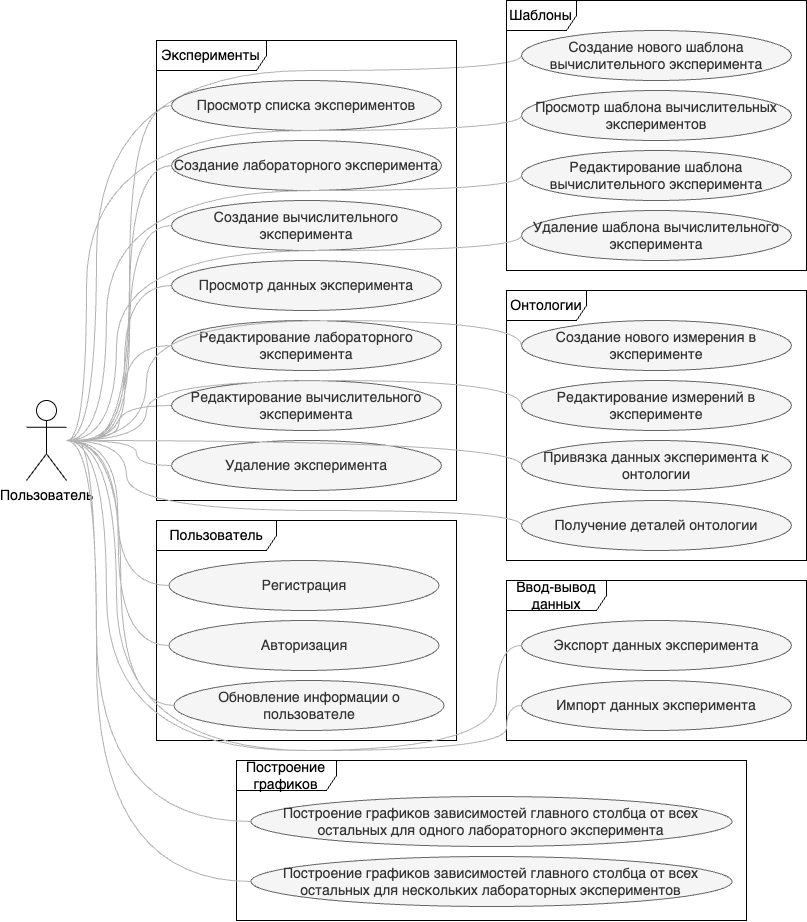
\includegraphics[width=0.5\linewidth]{img/use_cases.png}
    \caption{Диаграмма пользовательских сценариев}
    \label{pic:uc}
\end{figure}

\subsection{Архитектура приложения}

\subsubsection{Схема базы данных}

Таблица \texttt{users} хранит информацию о пользователях системы. Поле \texttt{id} является уникальным идентификатором пользователя. \texttt{username} содержит имя пользователя, а \texttt{username} — его уникальный никнейм. \texttt{hashed\_password} используется для хранения зашифрованного пароля. Поле \texttt{role} указывает на роль пользователя в системе.

Таблица \texttt{lab\_experiments} предназначена для хранения лабораторных экспериментов. \texttt{id} — уникальный идентификатор эксперимента. \texttt{title} содержит название эксперимента, а \texttt{description} — его описание. Поле \texttt{user\_id} указывает на пользователя, создавшего эксперимент. \texttt{created\_at} фиксирует дату и время создания записи.

Таблица \texttt{measurement} используется для хранения результатов измерений в лабораторных экспериментах. \texttt{id} — уникальный идентификатор записи. \texttt{experiment\_id} указывает, к какому лабораторному эксперименту относится измерение. \texttt{pivot\_key} определяет категорию данных. \texttt{parameter} хранит название измеряемого параметра, \texttt{value} содержит его числовое или текстовое значение. Поле \texttt{unit} связано с таблицей \texttt{ontology} и определяет единицу измерения.

Таблица \texttt{ontology} предназначена для хранения онтологических данных. Поле \texttt{id} является уникальным идентификатором онтологического термина. \texttt{name} содержит название термина, \texttt{dimension} — его размерность (например, масса, длина), а \texttt{uri} — ссылку на онтологический ресурс.

Таблица \texttt{computational\_experiments} хранит вычислительные эксперименты. \texttt{id} — уникальный идентификатор. \texttt{title} содержит название, а \texttt{description} — описание эксперимента. \texttt{user\_id} указывает на владельца эксперимента. Поле \texttt{created\_at} фиксирует дату создания, а \texttt{template\_id} связывает эксперимент с шаблоном из таблицы \texttt{computational\_templates}.

Таблица \texttt{computational\_experiment\_data} содержит конкретные данные вычислительных экспериментов. Поле \texttt{experiment\_id} связывает данные с конкретным экспериментом. \texttt{input\_data} хранит входные данные в формате JSON. \texttt{output\_data} содержит выходные данные, \texttt{parameters} включают параметры модели, а \texttt{context} — дополнительные сведения, не привязанные к онтологиям.

Таблица \texttt{computational\_templates} определяет шаблоны вычислительных экспериментов. Поле \texttt{id} является уникальным идентификатором, а \texttt{title} содержит название шаблона.

Таблица \texttt{computational\_experiment\_schemas} описывает схемы данных для вычислительных экспериментов. Поле \texttt{template\_id} связывает схему с соответствующим шаблоном. \texttt{input\_schema} определяет структуру входных данных в формате JSON, \texttt{output\_schema} — выходных, \texttt{parameter\_schema} описывает параметры эксперимента, а \texttt{context\_schema} задает структуру дополнительных данных.

Общая схема базы данных представлена на рисунке \ref{pic:db}.

\begin{figure}[H]
	\centering
	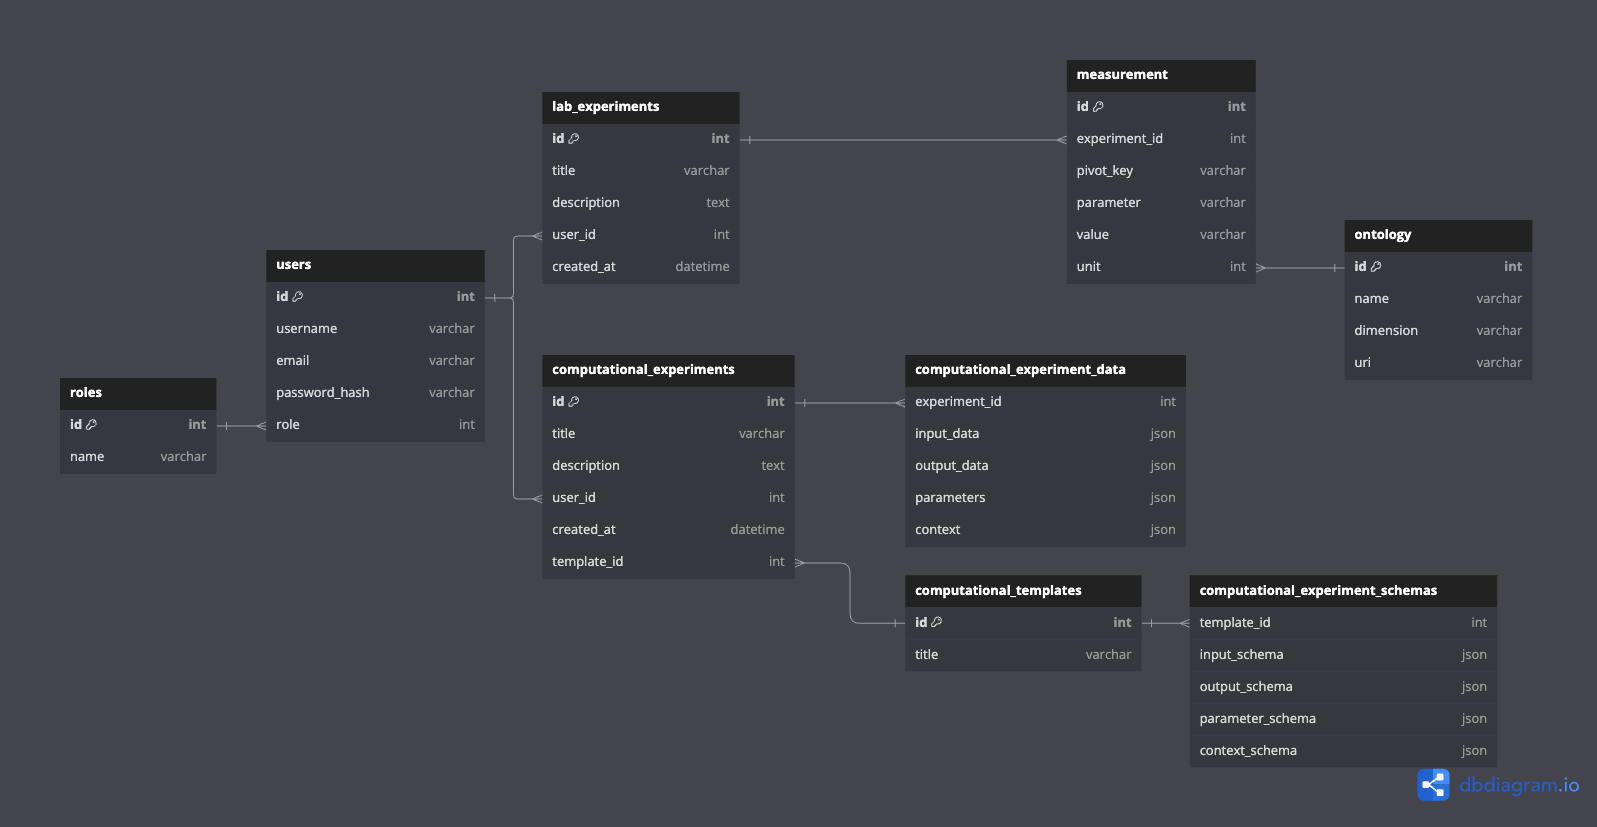
\includegraphics[width=\linewidth]{chapters/img/database_scheme.png}
	\caption{Схема базы данных}
	\label{pic:db}
\end{figure}


\subsubsection{Архитектура серверного приложения}

Выбранная архитектура приложения изображена на рисунке \ref{pic:server_arch} и основана на слоистом подходе, который обеспечивает разделение ответственности между компонентами, улучшает модульность и делает систему более поддерживаемой и масштабируемой. В серверной части реализована организация слоев: API Router обрабатывает входящие HTTP-запросы и передает их в слой бизнес-логики, где осуществляется основная обработка данных. Для работы с базами данных используется слой доступа к данным, который взаимодействует с PostgreSQL и Neo4j. Дополнительно выделены сервис аутентификации и уровень валидации, что обеспечивает безопасность и корректность данных.

\begin{figure}[H]
	\centering
	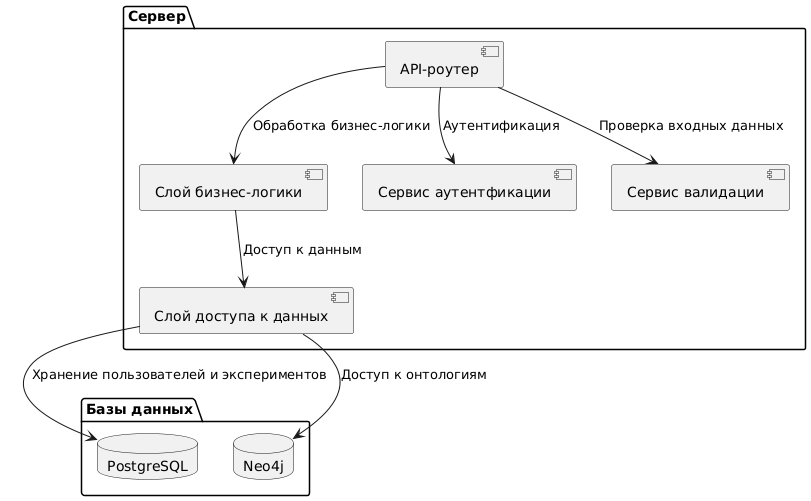
\includegraphics[width=0.7\linewidth]{chapters/img/server_arch.png}
	\caption{Архитектура серверного приложения}
	\label{pic:server_arch}
\end{figure}

\subsubsection{Архитектура клиентского приложения}

Клиентская часть построена на Vue.js и также следует принципам разделения ответственности. Компоненты пользовательского интерфейса взаимодействуют с хранилищем состояния (Pinia\cite{Library:Pinia}), которое управляет данными и их синхронизацией. Взаимодействие с сервером осуществляется через API Service, что позволяет отделить сетевые запросы от логики компонентов, а Vue Router\cite{Library:VueRouter} управляет навигацией. Такой подход обеспечивает гибкость и удобство в разработке. Архитектура клиентской части изображена на рисунке \ref{pic:client_arch}.

\begin{figure}[H]
	\centering
	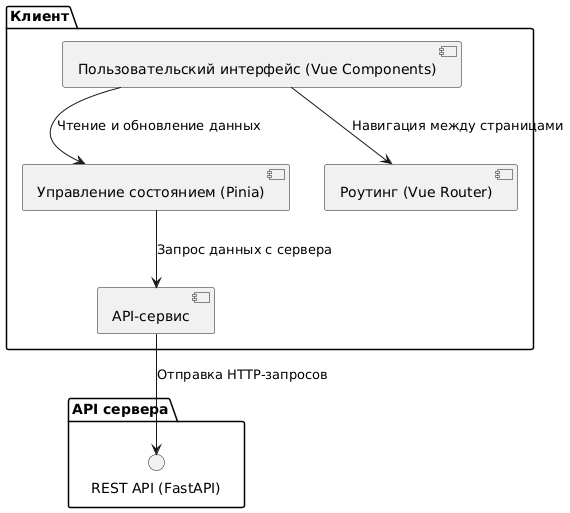
\includegraphics[width=\linewidth]{chapters/img/client_arch.png}
	\caption{Архитектура клиентского приложения}
	\label{pic:client_arch}
\end{figure}

\subsection{Выбор методов и средств реализации}

При выборе технологий для разработки веб-приложения учитывались следующие ключевые факторы:
\begin{enumerate}
    \item Производительность и масштабируемость.
    \item Простота интеграции с онтологиями.
    \item Поддержка современных стандартов веб-разработки.
    \item Лёгкость развертывания и сопровождения.
\end{enumerate}

На основании этих критериев были выбраны следующие технологии:

\subsubsection{Выбор фреймворка для серверной части}

В качестве веб-фреймворка для бэкенда было выбрано FastAPI по следующим причинам:
\begin{enumerate}
    \item Высокая производительность — благодаря использованию Starlette~\cite{Framework:Starlette} и Pydantic~\cite{Library:Pydantic}, FastAPI демонстрирует скорость работы, сопоставимую с Node.js~\cite{Lang:NodeJS} и Go~\cite{Lang:Go}, что особенно важно при работе с API для экспериментов.
    \item Асинхронная обработка запросов — поддержка async/await позволяет обрабатывать несколько запросов одновременно без блокировки потока выполнения, что критично при обработке вычислительных экспериментов.
    \item Встроенная валидация данных — благодаря Pydantic, валидация данных выполняется на уровне схем API, уменьшая вероятность ошибок на клиенте и сервере.
    \item Гибкость в интеграции — поддержка OpenAPI и облегчает документирование и подключение к клиентской части.
\end{enumerate}

Альтернативными вариантами были Django Rest Framework (DRF)~\cite{Framework:DRF} и Flask~\cite{Framework:Flask}, однако:
\begin{enumerate}
    \item DRF имеет более сложную архитектуру и высокие накладные расходы по сравнению с FastAPI.
    \item Flask не поддерживает асинхронную обработку из коробки, что снижает его эффективность для API с высокой нагрузкой.
\end{enumerate}

\subsubsection{Выбор фреймворка для клиентской части}

Для реализации фронтенда было выбрано Vue.js (Composition API) вместо React~\cite{Framework:React} и Angular~\cite{Framework:Angular}. Основные причины выбора:
\begin{enumerate}
    \item Лёгкость освоения и высокая продуктивность — Vue.js имеет интуитивно понятный синтаксис и гибкость в использовании как декларативного программирования, так и компонентов.
    \item Композиционный API — использование Composition API в Vue 3 улучшает переиспользуемость кода и упрощает управление состоянием.
    \item Высокая производительность — виртуальный DOM оптимизирован, механизм реактивности позволяет минимизировать ререндеринг.
    \item Гибкость в архитектуре — Vue.js легко интегрируется с серверными приложениями через REST API.
\end{enumerate}

Альтернативами рассматривались:
\begin{enumerate}
    \item React — мощный, но требует дополнительной конфигурации и использования сторонних библиотек для маршрутизации и управления состоянием.
    \item Angular — мощный, но имеет высокие накладные расходы на разработку.
\end{enumerate}

\subsubsection{Выбор библиотеки для пользовательского интерфейса}

Библиотека компонентов PrimeVue~\cite{Framework:PrimeVue} выбрана для реализации интерфейса по следующим причинам:
\begin{enumerate}
    \item Готовые UI-компоненты — ускоряет разработку благодаря наличию таблиц, форм, модальных окон и других элементов.
    \item Поддержка тем — пакет предоставляет несколько готовых тем, позволяющих легко менять визуальное оформление.
    \item Гибкость — компоненты адаптируются под мобильные и десктопные устройства.
\end{enumerate}

Альтернативой был Vuetify, но он менее гибок по сравнению с PrimeVue.

\subsubsection{Выбор реляционной СУБД}

В качестве основной базы данных была выбрана PostgreSQL, поскольку:
\begin{enumerate}
    \item Поддерживает сложные реляционные структуры — идеально подходит для хранения экспериментов, пользователей и привязок к онтологиям.
    \item Расширенные возможности JSONB — позволяет эффективно хранить и обрабатывать JSON-документы без использования NoSQL-решений.
    \item Высокая производительность — оптимизированные индексы и транзакции позволяют обрабатывать большие объёмы данных.
\end{enumerate}

Наиболее конкурентоспособная альтернатива – MySQL~\cite{DB:MySQL}, но данная СУБД хуже работает с JSONB и менее стабилен при высоких нагрузках.

\subsubsection{Выбор графовой СУБД}

Так как приложение активно работает с онтологиями, было принято решение использовать Neo4j для хранения и обработки онтологических связей:
\begin{enumerate}
    \item Графовая структура — идеально подходит для представления онтологий, где между сущностями существует множество взаимосвязей.
    \item Cypher Query Language~\cite{QueryLang:CypherQL} — позволяет легко выполнять сложные запросы, например, нахождение зависимостей между измерениями.
    \item Гибкость — позволяет расширять базу знаний без нарушения структуры данных.
    \item Плагин neosemantics~\cite{Library:NeoSemantics} – позволяет удобно работать с онтологиями, представленными в RDF/XML.
\end{enumerate}

\subsubsection{Выбор средств развёртывания}

Для контейнеризации приложения используется Docker Compose~\cite{Tool:DockerCompose}, по следующим причинам:
\begin{enumerate}
    \item Простота конфигурации — управление контейнерами через docker-compose.yml не требует сложных манифестов.
    \item Более удобен для разработки — локальная среда легко воспроизводится на разных машинах.
    \item Не требует дополнительного оркестратора — Kubernetes~\cite{Tool:Kubernetes} сложен в настройке и требует значительных ресурсов.
    \item Быстрое развертывание — приложение запускается одной командой, обеспечивая автоматический запуск всех сервисов.
\end{enumerate}

Kubernetes рассматривался как альтернатива, но его сложность оправдана только для высоконагруженных распределённых систем, что не является текущей целью проекта.

\anonsubsection{Выводы по главе}

В этой главе рассмотрены сценарии использования системы и её архитектура на разных уровнях. Подробно описана структура компонентов, их взаимодействие, а также ключевые аспекты разработки, включая выбор технологий и проектные решения.

    \setcounter{section}{3}
\setcounter{subsection}{0}
\sectionVKR{Программная реализация} \label{sec: 3}

В данной главе подробно рассматриваются принципы и подходы, применённые при реализации системы.
Описывается структура проекта, реализация логики на сервере, а также построение интерфейса.
Кроме этого, внимание уделяется механизмам работы с онтологиями и таблицами измерений, тестированию, развёртыванию и настройке окружения.
Все аспекты реализации подкреплены выбранными архитектурными решениями, описанными в предыдущей главе.

\subsection{Общая архитектура клиент-серверного приложения}

Приложение построено по клиент-серверной архитектуре, где фронтенд и бэкенд взаимодействуют через REST API. Данное решение позволяет обеспечивать масштабируемость, гибкость разработки и упрощённую интеграцию с различными внешними сервисами, включая онтологии OM2 и СhEBI.

На верхнем уровне приложение разделяется на три основных слоя:
\begin{enumerate}
    \item Клиентская часть -- реализована на Vue.js с использованием PrimeVue, Pinia для управления состоянием и Vue Router для маршрутизации.
    \item Серверная часть -- написана на FastAPI, использует SQLAlchemy~\cite{Library:SQLAlchemy} для работы с базой данных, Alembic~\cite{Library:Alembic} для управления миграциями и JWT для аутентификации.
    \item Базы данных -- в качестве реляционной СУБД используется PostgreSQL в которой хранятся все данные пользователей, экспериментов и привязок к онтологиям, а в качестве графовой -- Neo4j для хранения полной информации о доступных для использованию онтологиях.
\end{enumerate}

\subsection{Архитектурные паттерны и подходы}

Для структурирования кода и повышения удобочитаемости используются следующие архитектурные паттерны:

\begin{enumerate}
    \item MVVM (Model-View-ViewModel) -- используется во Vue.js для упрощения двустороннего связывания данных между представлением и логикой.
    \item ORM (Object-Relational Mapping) -- SQLAlchemy используется как ORM для работы с реляционной базой данных PostgreSQL.
%    \item RESTful API -- бэкенд реализует REST API, обеспечивающий взаимодействие с клиентской частью и внешними сервисами.
\end{enumerate}

\subsection{Выбор технологий}

Выбор технологий осуществлялся с учётом специфики проекта: необходимости работы с онтологиями, хранения сложных структур данных в формате JSON, реализации гибкого пользовательского интерфейса, масштабируемости и удобства сопровождения.
Ниже приведён список использованных инструментов с обоснованием их выбора.

FastAPI выбран вместо Django и Flask, так как обеспечивает асинхронную обработку запросов, полностью совместим с Pydantic, используется в связке с SQLAlchemy, а также предоставляет автогенерацию документации по API, что существенно упрощает отладку и интеграцию с фронтендом.

SQLAlchemy используется в качестве ORM-библиотеки, так как позволяет точно контролировать структуру базы данных, реализовать наследование и сложные связи между таблицами, а также поддерживает асинхронные операции, что критично для работы с FastAPI.

Alembic применяется для управления миграциями, так как является официальным решением для SQLAlchemy и позволяет отслеживать изменения схемы базы данных в виде версионированных скриптов.

Pydantic используется для описания и валидации входных и выходных структур API. Он был выбран благодаря строгой типизации и глубокой интеграции с FastAPI, что позволяет обеспечить безопасность данных на уровне схем.

Vue выбран вместо React из-за необходимости сторонних решений для маршрутизации и хранения состояния у последнего.

PrimeVue выбран вместо Vuetify, так как не навязывает Material Design, поддерживает Tailwind CSS~\cite{Library:TailwindCSS}, а также предоставляет компонент TreeTable, который критичен для отображения иерархии экспериментов и отсутствует в Vuetify.

Pinia используется вместо Vuex, поскольку лучше интегрируется с Composition API, не требует шаблонного кода и обеспечивает типобезопасную работу с глобальным состоянием.

Axios~\cite{Library:Axios} выбран для выполнения HTTP-запросов вместо Fetch API, так как предоставляет более удобный механизм перехвата запросов, централизованную обработку ошибок и простую интеграцию с системой авторизации.

PostgreSQL выбран в качестве основной базы данных, поскольку поддерживает бинарный формат JSONB, который идеально подходит для хранения входных и выходных структур вычислительных экспериментов. Также PostgreSQL обеспечивает надёжную реализацию внешних ключей, каскадного удаления и индексов, включая поддержку рекурсивных запросов и типизацию ENUM.

Neo4j используется для хранения онтологий, так как предоставляет графовую модель, наиболее естественную для представления онтологических связей.
Благодаря расширению neosemantics (n10s) возможна загрузка RDF-графов и выполнение Cypher-запросов к онтологиям.
Использование альтернативных решений на Java было бы избыточным по сравнению с лёгкой интеграцией Neo4j в стек Python.

Docker~\cite{Tool:Docker} и Docker Compose применяются для контейнеризации приложения и управления зависимостями между сервисами.
Это обеспечивает повторяемость окружения и упрощает развёртывание.

Nginx~\cite{Tool:Nginx} используется в качестве обратного прокси-сервера благодаря своей простоте и стабильности.

\subsection{Разработка серверной части}

В качестве основы использован фреймворк FastAPI, благодаря которому реализована быстрая и типобезопасная работа с REST API.
Для работы с реляционной базой данных PostgreSQL применялась SQLAlchemy, а миграции выполнялись с помощью Alembic.
Модели базы данных были спроектированы с учётом использования ENUM, каскадных удалений и связей между таблицами, отражающих структуру предметной области.
Отдельное внимание уделено работе с онтологиями -- для этого реализована интеграция с графовой базой данных Neo4j, обеспечивающей доступ к элементам онтологий через обёртку для Cypher-запросов.
С точки зрения архитектурных решений, сервер был спроектирован как набор модулей, разделённых по областям ответственности: маршруты, схемы запросов/ответов, бизнес-логика и работа с БД.
Это упрощает расширение и сопровождение системы.

\subsubsection{Структура серверного приложения}

Кодовая база серверной части организована следующим образом:

\begin{enumerate}
\item \texttt{alembic} -- пакет с настройками инструмента Alembic и миграциями базы данных.
\item \texttt{models} -- пакет с ORM-моделями базы данных, описанные с использованием SQLAlchemy, а также кодом для работы с онтологиями.
\item \texttt{config} -- папка с настройками приложения для трёх разных окружений -- разработки, тестирования и продакшена.
\item \texttt{ontology} -- пакет с вспомогательными утилитами для работы с графовой СУБД Neo4j и языком запросов Cypher.
\item \texttt{routes} -- пакет с обработчиками HTTP-запросов, организованными в соответствии с REST API.
\item \texttt{services} -- пакет с бизнес-логикой приложения, отделённой от маршрутов.
\item \texttt{schemas} -- пакет Pydantic-схемы для валидации входных и выходных данных API.
\item \texttt{tests} -- пакет с тестами.
\item \texttt{config.py} -- файл конфигурации приложения, загружающий переменные окружения и производящий прочие настройки.
\end{enumerate}

\subsubsection{Модели базы данных}\label{ORM models}

Данные в приложении хранятся в PostgreSQL. Для работы с базой данных используется ORM SQLAlchemy. Основные сущности базы данных:

\begin{enumerate}
\item \texttt{User} -- хранит данные о пользователях.
\item \texttt{Profile} -- расширяет информацию о пользователе.
\item \texttt{Experiment} -- базовая таблица для всех экспериментов, содержащая описание, путь к файлу и временные метки.
\item \texttt{LaboratoryExperiment} -- конкретизация \texttt{Experiment}, привязанная к пользователю и содержащая измерения и описание столбцов.
\item \texttt{Measurement} -- хранит данные измерений, относящиеся к лабораторному эксперименту.
\item \texttt{Column} -- описание столбцов эксперимента с привязкой к онтологиям.
\item \texttt{Schema} -- хранит JSON-данные входов, выходов, параметров и контекста эксперимента.
\item \texttt{ComputationalExperiment} -- вычислительный эксперимент, связанный с шаблоном и входными/выходными данными.
\item \texttt{ComputationalExperimentTemplate} -- шаблон вычислительного эксперимента, содержащий связанные эксперименты.
\item \texttt{ComputationalExperimentData} -- данные вычислительного эксперимента, связанные с конкретным экспериментом.
\end{enumerate}

Вспомогательные классы, расширяющие возможности основных сущностей или упрощающие работу с ними:

\begin{enumerate}
\item \texttt{PathMixin} -- используется для всех сущностей, имеющих поле \texttt{path}.
\item \texttt{OwnableMixin} -- используется для всех сущностей, привязанных к пользователю.
\item \texttt{SchemaLinkedTableMixin} -- используется для связи таблиц с таблицей схем (\texttt{Schema}).
\end{enumerate}

\subsubsection{Реализация API для работы с экспериментами}

API реализовано в соответствии с RESTful-архитектурой.
Далее в отдельных разделах описаны эндпоинты.

\paragraph{Эндпоинты аутентификации}

\begin{enumerate}
\item \texttt{POST /auth/signup} -- регистрация нового пользователя.
\begin{enumerate}[label=\arabic{enumi}.\arabic*.]
\item Входные данные: \texttt{UserSignup} (имя пользователя, роль, пароль).
\item Ответ: сообщение о регистрации.
\end{enumerate}

\item \texttt{POST /auth/signin} -- вход в систему, возвращает access и refresh токены.
\begin{enumerate}[label=\arabic{enumi}.\arabic*.]
\item Входные данные: \texttt{UserLogin} (имя пользователя, пароль).
\item Ответ: объект \texttt{UserResponse}, содержащий \texttt{access\_token} и \texttt{refresh\_token}.
\end{enumerate}

\item \texttt{POST /auth/refresh} -- обновление access/refresh токенов.
\begin{enumerate}[label=\arabic{enumi}.\arabic*.]
\item Входные данные: refresh-токен.
\item Ответ: новый \texttt{access\_token} и \texttt{refresh\_token}.
\end{enumerate}
\end{enumerate}

\paragraph{Эндпоинты профиля}

\begin{enumerate}
\item \texttt{GET /user/profile} -- получение профиля текущего пользователя.
\begin{enumerate}[label=\arabic{enumi}.\arabic*.]
\item Выходные данные: \texttt{ProfileResponse} (содержит username, name, surname, email, position, registered\_at, last\_login и список экспериментов).
\end{enumerate}
\item \texttt{PATCH /user/profile} -- обновление полей профиля текущего пользователя.
\begin{enumerate}[label=\arabic{enumi}.\arabic*.]
\item Входные данные: \texttt{ProfileUpdateRequest} (любой набор полей: username, name, surname, position, email).
\item Выходные данные: обновлённый \texttt{ProfileResponse}.
\end{enumerate}
\end{enumerate}

\paragraph{Эндпоинты управления экспериментами}

\begin{enumerate}
\item \texttt{GET /experiment/} -- получение списка экспериментов пользователя.
\begin{enumerate}[label=\arabic{enumi}.\arabic*.]
\item Входные параметры: \texttt{desired\_keys} (список ключей).
\item Ответ: список данных о экспериментах.
\end{enumerate}

\item \texttt{GET /experiment/{experiment\_id}} -- получение данных конкретного эксперимента.
\begin{enumerate}[label=\arabic{enumi}.\arabic*.]
\item Входные параметры: \texttt{experiment\_id} (идентификатор эксперимента).
\item Ответ: данные лабораторного или вычислительного эксперимента.
\end{enumerate}

\item \texttt{POST /experiment/laboratory} -- создание лабораторного эксперимента.
\begin{enumerate}[label=\arabic{enumi}.\arabic*.]
\item Входные данные: \texttt{CreateLaboratoryExperimentRequest}.
\item Ответ: объект \texttt{LaboratoryExperimentDetails}.
\end{enumerate}

\item \texttt{POST /experiment/computational} -- создание вычислительного эксперимента.
\begin{enumerate}[label=\arabic{enumi}.\arabic*.]
\item Входные данные: \texttt{CreateComputationalExperimentRequest}.
\item Ответ: объект \texttt{ComputationalExperimentDetails}.
\end{enumerate}

\item \texttt{PATCH /experiment/laboratory/{experiment\_id}} -- обновление лабораторного эксперимента.
\begin{enumerate}[label=\arabic{enumi}.\arabic*.]
\item Входные параметры: \texttt{experiment\_id} (идентификатор эксперимента).
\item Входные данные: \texttt{UpdateLaboratoryExperimentRequest}.
\item Ответ: обновленные данные лабораторного эксперимента.
\end{enumerate}

\item \texttt{PATCH /experiment/computational/{experiment\_id}} -- обновление вычислительного эксперимента.
\begin{enumerate}[label=\arabic{enumi}.\arabic*.]
\item Входные параметры: \texttt{experiment\_id} (идентификатор эксперимента).
\item Входные данные: \texttt{UpdateComputationalExperimentRequest}.
\item Ответ: обновленные данные вычислительного эксперимента.
\end{enumerate}

\item \texttt{DELETE /experiment/{experiment\_id}} -- удаление эксперимента.
\begin{enumerate}[label=\arabic{enumi}.\arabic*.]
\item Входные параметры: \texttt{experiment\_id} (идентификатор эксперимента).
\item Ответ: сообщение об успешном удалении.
\end{enumerate}
\end{enumerate}

\paragraph{Эндпоинты импорта и экспорта экспериментов}

\begin{enumerate}
\item \texttt{GET /experiment/export/\{experiment\_id\}} -- экспорт данных эксперимента.
\begin{enumerate}[label=\arabic{enumi}.\arabic*.]
\item Входные параметры: \texttt{experiment\_id} (идентификатор эксперимента), \texttt{export\_type} – формат экспорта ('json' или 'xml').
\item Ответ: скачиваемый файл с данными эксперимента в формате JSON или XML.
\end{enumerate}
\item \texttt{POST /experiment/import/laboratory} -- импорт лабораторного эксперимента из JSON.
\begin{enumerate}[label=\arabic{enumi}.\arabic*.]
\item Входные данные: формат подробно описан в Приложении А (техническое задание).
\item Ответ: данные созданного лабораторного эксперимента.
\end{enumerate}
\item \texttt{POST /experiment/import/computational} -- импорт вычислительного эксперимента из JSON.
\begin{enumerate}[label=\arabic{enumi}.\arabic*.]
\item Входные данные: формат подробно описан в Приложении А (техническое задание).
\item Ответ: данные созданного вычислительного эксперимента.
\end{enumerate}
\end{enumerate}

\paragraph{Эндпоинты работы с онтологиями}

\begin{enumerate}
\item \texttt{GET /ontology/} -- получение списка доступных онтологий.
\begin{enumerate}[label=\arabic{enumi}.\arabic*.]
\item Ответ: список всех онтологий с базовой информацией.
\end{enumerate}

\item \texttt{GET /ontology/details/{ontology}} -- получение подробной информации о конкретной онтологии.
\begin{enumerate}[label=\arabic{enumi}.\arabic*.]
\item Входные параметры: \texttt{ontology} (имя онтологии), \texttt{limit} (ограничение на количество элементов).
\item Ответ: подробности об указанной онтологии.
\end{enumerate}
\end{enumerate}

\paragraph{Эндпоинты работы с шаблонами вычислительных экспериментов}

\begin{enumerate}
\item \texttt{GET /template/} -- получение списка шаблонов вычислительных экспериментов.
\begin{enumerate}[label=\arabic{enumi}.\arabic*.]
\item Ответ: список доступных шаблонов.
\end{enumerate}

\item \texttt{POST /template/} -- создание нового шаблона для вычислительного эксперимента.
\begin{enumerate}[label=\arabic{enumi}.\arabic*.]
\item Входные данные: \texttt{CreateTemplateRequest}.
\item Ответ: объект \texttt{TemplateDetails} (данные созданного шаблона).
\end{enumerate}

\item \texttt{GET /template/{template\_id}} -- получение данных конкретного шаблона.
\begin{enumerate}[label=\arabic{enumi}.\arabic*.]
\item Входные параметры: \texttt{template\_id} (идентификатор шаблона).
\item Ответ: данные шаблона.
\end{enumerate}

\item \texttt{PATCH /template/{template\_id}} -- обновление шаблона.
\begin{enumerate}[label=\arabic{enumi}.\arabic*.]
\item Входные параметры: \texttt{template\_id} (идентификатор шаблона).
\item Входные данные: \texttt{UpdateTemplateRequest}.
\item Ответ: обновленные данные шаблона.
\end{enumerate}

\item \texttt{DELETE /template/{template\_id}} -- удаление шаблона.
\begin{enumerate}[label=\arabic{enumi}.\arabic*.]
\item Входные параметры: \texttt{template\_id} (идентификатор шаблона).
\item Ответ: сообщение об успешном удалении шаблона.
\end{enumerate}
\end{enumerate}

\subsubsection{Аутентификация и авторизация пользователей}

Для управления доступом используется аутентификация на основе JWT.
Пользователь после успешного входа получает короткоживущий access-токен, позволяющий получить доступ к ресурсам системы, и refresh-токен, в течение жизни которого можно перевыпустить access-токен.
Если срок жизни refresh-токена истекает, требуется повторная авторизация с указанием имени пользователя и пароля.

При каждом запросе к защищённым маршрутам проверяется валидность токена.

\subsubsection{Работа с онтологиями}

Для работы с онтологиями используется интеграция с OM2 и СhEBI.
Приложение позволяет привязывать столбцы таблиц экспериментов к онтологиям, что упрощает интерпретацию данных.

\begin{enumerate}
\item Поддерживается хранение привязок к онтологиям через таблицу \texttt{ColumnDescription}.
\item Используется Neo4j для представления связей между сущностями онтологий.
\item Запросы к онтологиям выполняются с использованием языка Cypher (пример в листинге~\ref{lst:Cypher0}).
\end{enumerate}

\begin{lstlisting}[frame=single, basicstyle=\footnotesize\ttfamily, label={lst:Cypher0}, caption={Пример запроса к Neo4j для поиска онтологических связей},captionpos=b, breaklines=true, breakatwhitespace=true]

MATCH (m:Measurement)-[:HAS_UNIT]->(u:Unit)
WHERE m.name = "length"
RETURN u.name
\end{lstlisting}

\subsubsection{Логирование и обработка ошибок}

Для мониторинга работы сервера используется система логирования.
Основные особенности:

\begin{enumerate}
\item Логи ошибок записываются в файл \texttt{logs/errors.log}.
\item Информация о запросах и ответах записывается в консоль.
\end{enumerate}

\subsection{Разработка клиентской части}

\subsubsection{Общая структура фронтенда}

Клиентская часть веб-приложения разработана с использованием фреймворка Vue.js, который обеспечивает удобное построение интерфейсов и модульную организацию кода.
В проекте используется Composition API, что позволяет эффективно управлять состоянием приложения.

Основные технологии, применяемые во фронтенде:
\begin{enumerate}
\item Vue.js -- фреймворк для разработки пользовательских интерфейсов.
\item PrimeVue -- библиотека UI-компонентов.
\item Pinia -- инструмент для управления состоянием.
\item Vue Router -- система маршрутизации.
\item Axios -- библиотека для работы с API.
\end{enumerate}

Фронтенд структурирован следующим образом:
\begin{enumerate}
\item \texttt{src/main.ts} -- точка входа в приложение.
\item \texttt{src/router/index.ts} -- маршрутизация внутри приложения.
\item \texttt{src/stores/} -- хранилища состояния (Pinia).
\item \texttt{src/components/} -- простые компоненты.
\item \texttt{src/composable/} -- утилиты и композиции для переиспользуемой логики.
\item \texttt{src/api/axios.ts} -- конфигурация отправки API-запросов.
\item \texttt{src/views/} -- представления страниц.
\item \texttt{src/layout/} -- компоненты макета.
\end{enumerate}

\subsubsection{Компоненты и представления}

Фронтенд-приложение содержит набор компонентов и представлений, организованных в директориях \texttt{src/components} и \texttt{src/views}.
Компоненты обеспечивают переиспользуемые элементы интерфейса, а представления реализуют основные страницы приложения.

\paragraph{Компоненты}

\begin{enumerate}
\item \texttt{Editor} -- компонент редактора текста, используемый для ввода описаний экспериментов.
\begin{enumerate}[label=\arabic{enumi}.\arabic*.]
\item Входные параметры: \texttt{description} (текст описания).
\item Выходные параметры: обновленный текст.
\end{enumerate}

\item \texttt{FloatingConfigurator} -- компонент конфигуратора, который позволяет изменять настройки отображения данных.
\begin{enumerate}[label=\arabic{enumi}.\arabic*.]
\item Входные параметры: \texttt{settings} (объект параметров конфигурации).
\item Выходные параметры: обновленный объект конфигурации.
\end{enumerate}

\item \texttt{Table} -- компонент таблицы для отображения результатов измерений.
\begin{enumerate}[label=\arabic{enumi}.\arabic*.]
\item Входные параметры: \texttt{columns} (информация о столбцах), \texttt{data} (информация о ячейках).
\item Выходные параметры: отредактированные данные.
\end{enumerate}
\end{enumerate}

\paragraph{Представления}

\begin{enumerate}
\item \texttt{Auth/SignIn} -- страница входа в систему.
\item \texttt{Auth/SignUp} -- страница регистрации нового пользователя.
\item \texttt{Dashboard/CreateExperimentDialog} -- диалог создания нового эксперимента.
\item \texttt{Dashboard/CreateFolderDialog} -- диалог создания новой папки.
\item \texttt{Dashboard/Dashboard} -- главная страница дашборда.
\item \texttt{Dashboard/ExperimentActions} -- панель действий над экспериментом (удаление, перемещение и т.д.).
\item \texttt{Dashboard/ExperimentTable} -- таблица всех доступных экспериментов.
\item \texttt{Dashboard/MoveDialog} -- диалог перемещения эксперимента или шаблона в другую папку.
\item \texttt{Dashboard/TemplateActions} -- панель действий над шаблоном (удаление, перемещение и т.д.)
\item \texttt{Dashboard/TemplateSchemaForm} -- встраиваемый компонент для просмотра схем шаблона вычислительного эксперимента.
\item \texttt{Dashboard/TemplateTable} -- таблица всех доступных шаблонов вычислительных экспериментов.
\item \texttt{Dashboard/ViewTemplateDialog} -- диалог для просмотра схем шаблона вычислительного эксперимента.
\item \texttt{Editors/LabExperiment/Charts} -- компонент для отображения графиков, связанных с данными лабораторного эксперимента.
\item \texttt{Editors/LabExperiment/EditColumnDialog} -- компонент для редактирования столбцов лабораторного эксперимента.
\item \texttt{Editors/LabExperiment/LabExperiment} -- основной компонент для редактирования и отображения лабораторного эксперимента, включая описание и таблицы.
\item \texttt{Editors/LabExperiment/Table} -- компонент для отображения таблицы данных лабораторного эксперимента.
\item \texttt{Editors/ComputationalExperiment} -- стораница редактирования вычислительного эксперимента.
\item \texttt{OntologyDetails/ChEBIDetails} -- компонент отображения подробной информации по онтологии ChEBI, включая список сущностей и их свойств.
\item \texttt{OntologyDetails/OM2Details} -- компонент отображения подробной информации по онтологии OM2, включая физические величины и единицы измерения.
\item \texttt{OntologyDetails/OntologyList} -- компонент, выводящий список всех доступных онтологий с возможностью выбора и навигации между ними.
\item \texttt{Utils/AccessDenied} -- страница ошибки доступа.
\item \texttt{Utils/Error} -- страница общей ошибки.
\item \texttt{Utils/NotFound} -- страница общей ошибки.
\item \texttt{Utils/Support} -- страница с контактной информацией.
\item \texttt{Explore} -- страница для сравнения данных нескольких лабораторных экспериментов с одинаковыми столбцами.
\end{enumerate}

Кроме самописных компонентов, для создания пользовательского интерфейса используются компоненты PrimeVue.
В том числе общие элементы интерфейса организованы построены с помощью:

\begin{enumerate}
\item \texttt{AppLayout} -- основной макет приложения, содержащий боковое меню (\texttt{AppSidebar}), навигационную панель (\texttt{AppTopbar}) и футер (подвал) (\texttt{AppFooter}).
\item \texttt{AppMenu} -- навигационное меню, содержащее основные ссылки.
\end{enumerate}

Все эти компоненты и представления работают вместе, формируя клиентскую часть приложения и обеспечивая удобный пользовательский интерфейс.

\subsubsection{Маршрутизация}

Веб-приложение использует систему маршрутизации Vue Router.
Ниже приведены основные маршруты:

\begin{enumerate}
\item \texttt{/} -- главная страница (панель управления экспериментами).
\item \texttt{/experiment/laboratory/\{id\}} -- страница редактирования лабораторного эксперимента.
\item \texttt{/experiment/computational/\{id\}} -- страница редактирования вычислительного эксперимента.
\item \texttt{/ontology} -- страница списка онтологий.
\item \texttt{/ontology/details/om2} -- страница подробной информации о онтологии OM2.
\item \texttt{/ontology/details/chebi} -- страница подробной информации о онтологии ChEBI.
\item \texttt{/support} -- страница c контактной информацией.
\item \texttt{/explore} -- страница для сравнения данных нескольких лабораторных экспериментов.
\item \texttt{/notfound} -- страница общей ошибки.
\item \texttt{/auth/signin} -- страница входа.
\item \texttt{/auth/signup} -- страница регистрации нового пользователя.
\item \texttt{/auth/accessdenied} -- страница ошибки доступа.
\end{enumerate}

Каждый маршрут связан с соответствующим представлением во фронтенде и управляется Vue Router, а переход на любой маршрут, не перечисленный выше, приведёт к переходу на страницу общей ошибки.

\subsubsection{Управление состоянием}

Для управления глобальным состоянием используется Pinia.
Этот пакет позволяет:

\begin{enumerate}
\item Глобально управлять состоянием без необходимости пробрасывания данных через длинную цепочку компонентов.
\item Обеспечивать предсказуемость данных, поскольку все изменения происходят через строго определённые методы.
\item Легко организовывать разделение логики в приложении, сохраняя состояние в отдельных модулях.
\item Хранить данные между разными страницами и компонентами, не теряя их при переходах.
\end{enumerate}

Приложение использует два хранилища:

\begin{enumerate}
\item \texttt{src/stores/core.ts} -- отвечает за глобальные настройки интерфейса и данные пользователя, которые могут потребоваться в любой части приложения.
\end{enumerate}

\subsubsection{Взаимодействие с API}

Для работы с API используется библиотека Axios.
Библиотека предоставляет удобный механизм перехватчиков (interceptors), позволяющих совершать манипуляции над каждым запросом перед его отправкой или результатом запроса после его завершения.
С помощью этого механизма настроены:
\begin{enumerate}
\item Автоматическое прикрепление access-токена в заголовок \texttt{Authorization}
\item Автоматическое обновление access-токена, если код ответа равен 401 (Unauthorized)
\end{enumerate}

\subsubsection{Редактирование экспериментов}

Редактирование экспериментов является одной из ключевых функций веб-приложения.
В системе предусмотрены отдельные представления для работы с лабораторными и вычислительными экспериментами.
Пользователь может изменять описание эксперимента, редактировать параметры и вносить изменения в таблицу результатов.

Редактирование лабораторного эксперимента осуществляется через интерфейс, содержащий текстовый редактор и таблицу данных (представлен на рис.~\ref{pic:lab_experiment_editor}).
Пользователь может изменять структуру эксперимента, добавлять или удалять столбцы, а также управлять привязками к онтологиям.

Для вычислительных экспериментов предусмотрены дополнительные возможности, такие как редактирование входных данных, параметров модели и контекстной информации.

Редактирование доступно только владельцам эксперимента.

\begin{figure}[H]
\centering
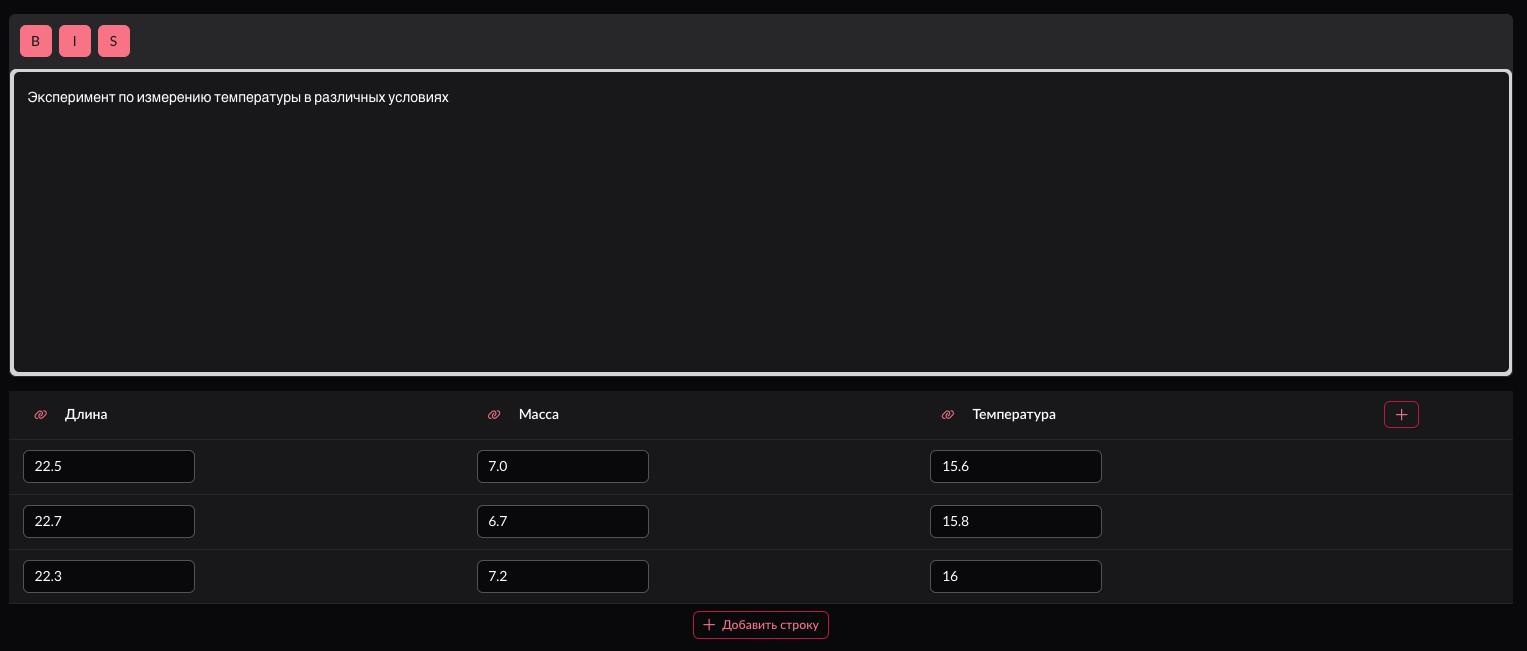
\includegraphics[width=\linewidth]{img/experiment_view.png}
\caption{Окно просмотра данных эксперимента}
\label{pic:lab_experiment_editor}
\end{figure}
\vspace{0.5cm}

\subsubsection{Таблица результатов измерений}

Таблица результатов измерений является важной частью экспериментов, позволяя пользователю фиксировать и анализировать полученные данные.
Каждая колонка таблицы может быть связана с определённой онтологией, что позволяет обеспечить корректную интерпретацию данных.

При редактировании эксперимента пользователь может задать для каждого столбца его онтологию и элемент онтологии, который этот столбец репрезентует.
Это облегчает обмен данными с другими системами.
Отображение таблицы реализовано в виде интерактивного компонента, который позволяет пользователям редактировать данные.

\subsubsection{Адаптивность и мобильная версия}

Интерфейс приложения адаптирован под мобильные устройства с использованием медиазапросов и классов Tailwind CSS (рис.~\ref{pic:mobile_version}).
Адаптивность обеспечивается настройками макета, темы, акцентного цвета и цвета фона (рис.~\ref{pic:other_colors}).

Благодаря этому при уменьшении ширины экрана боковая панель скрывается, а контент центрируется, а пользователи с особенностями зрения могут подобрать комфортное для них сочетание цветов и темы, делающее управляющие элементы сайта наиболее заметными, а работу комфортной.

\begin{figure}[H]
\centering
\begin{minipage}{0.45\linewidth}
\centering

\includegraphics[width=\linewidth]{img/mobile_version.png}
\caption{Окно просмотра данных эксперимента}
\label{pic:mobile_version}
\end{minipage}\hfill
\begin{minipage}{0.45\linewidth}
\centering
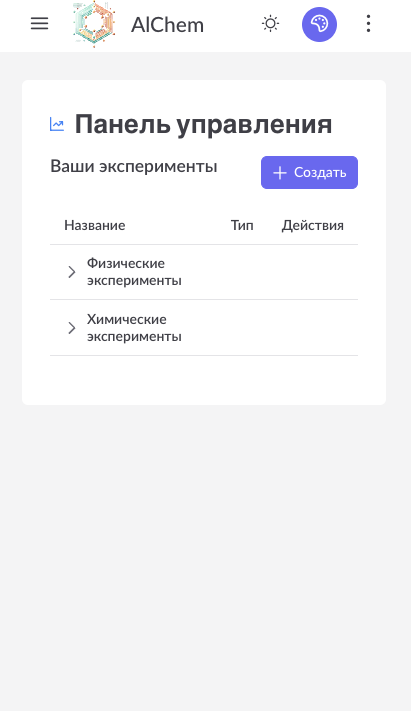
\includegraphics[width=\linewidth]{img/other_colors.png}
\caption{Выбор других сочетаний цветов и темы}
\label{pic:other_colors}
\end{minipage}
\end{figure}
\vspace{0.5cm}

\subsection{Работа с базой данных}

\subsubsection{Структура базы данных и схемы таблиц}

В качестве основной СУБД используется PostgreSQL, обеспечивающая высокую надёжность и поддержку сложных реляционных связей.
Схема базы данных (рис.~\ref{pic:postgres_scheme}) организована таким образом, чтобы минимизировать дублирование данных и оптимизировать запросы.

\begin{figure}[H]
\centering
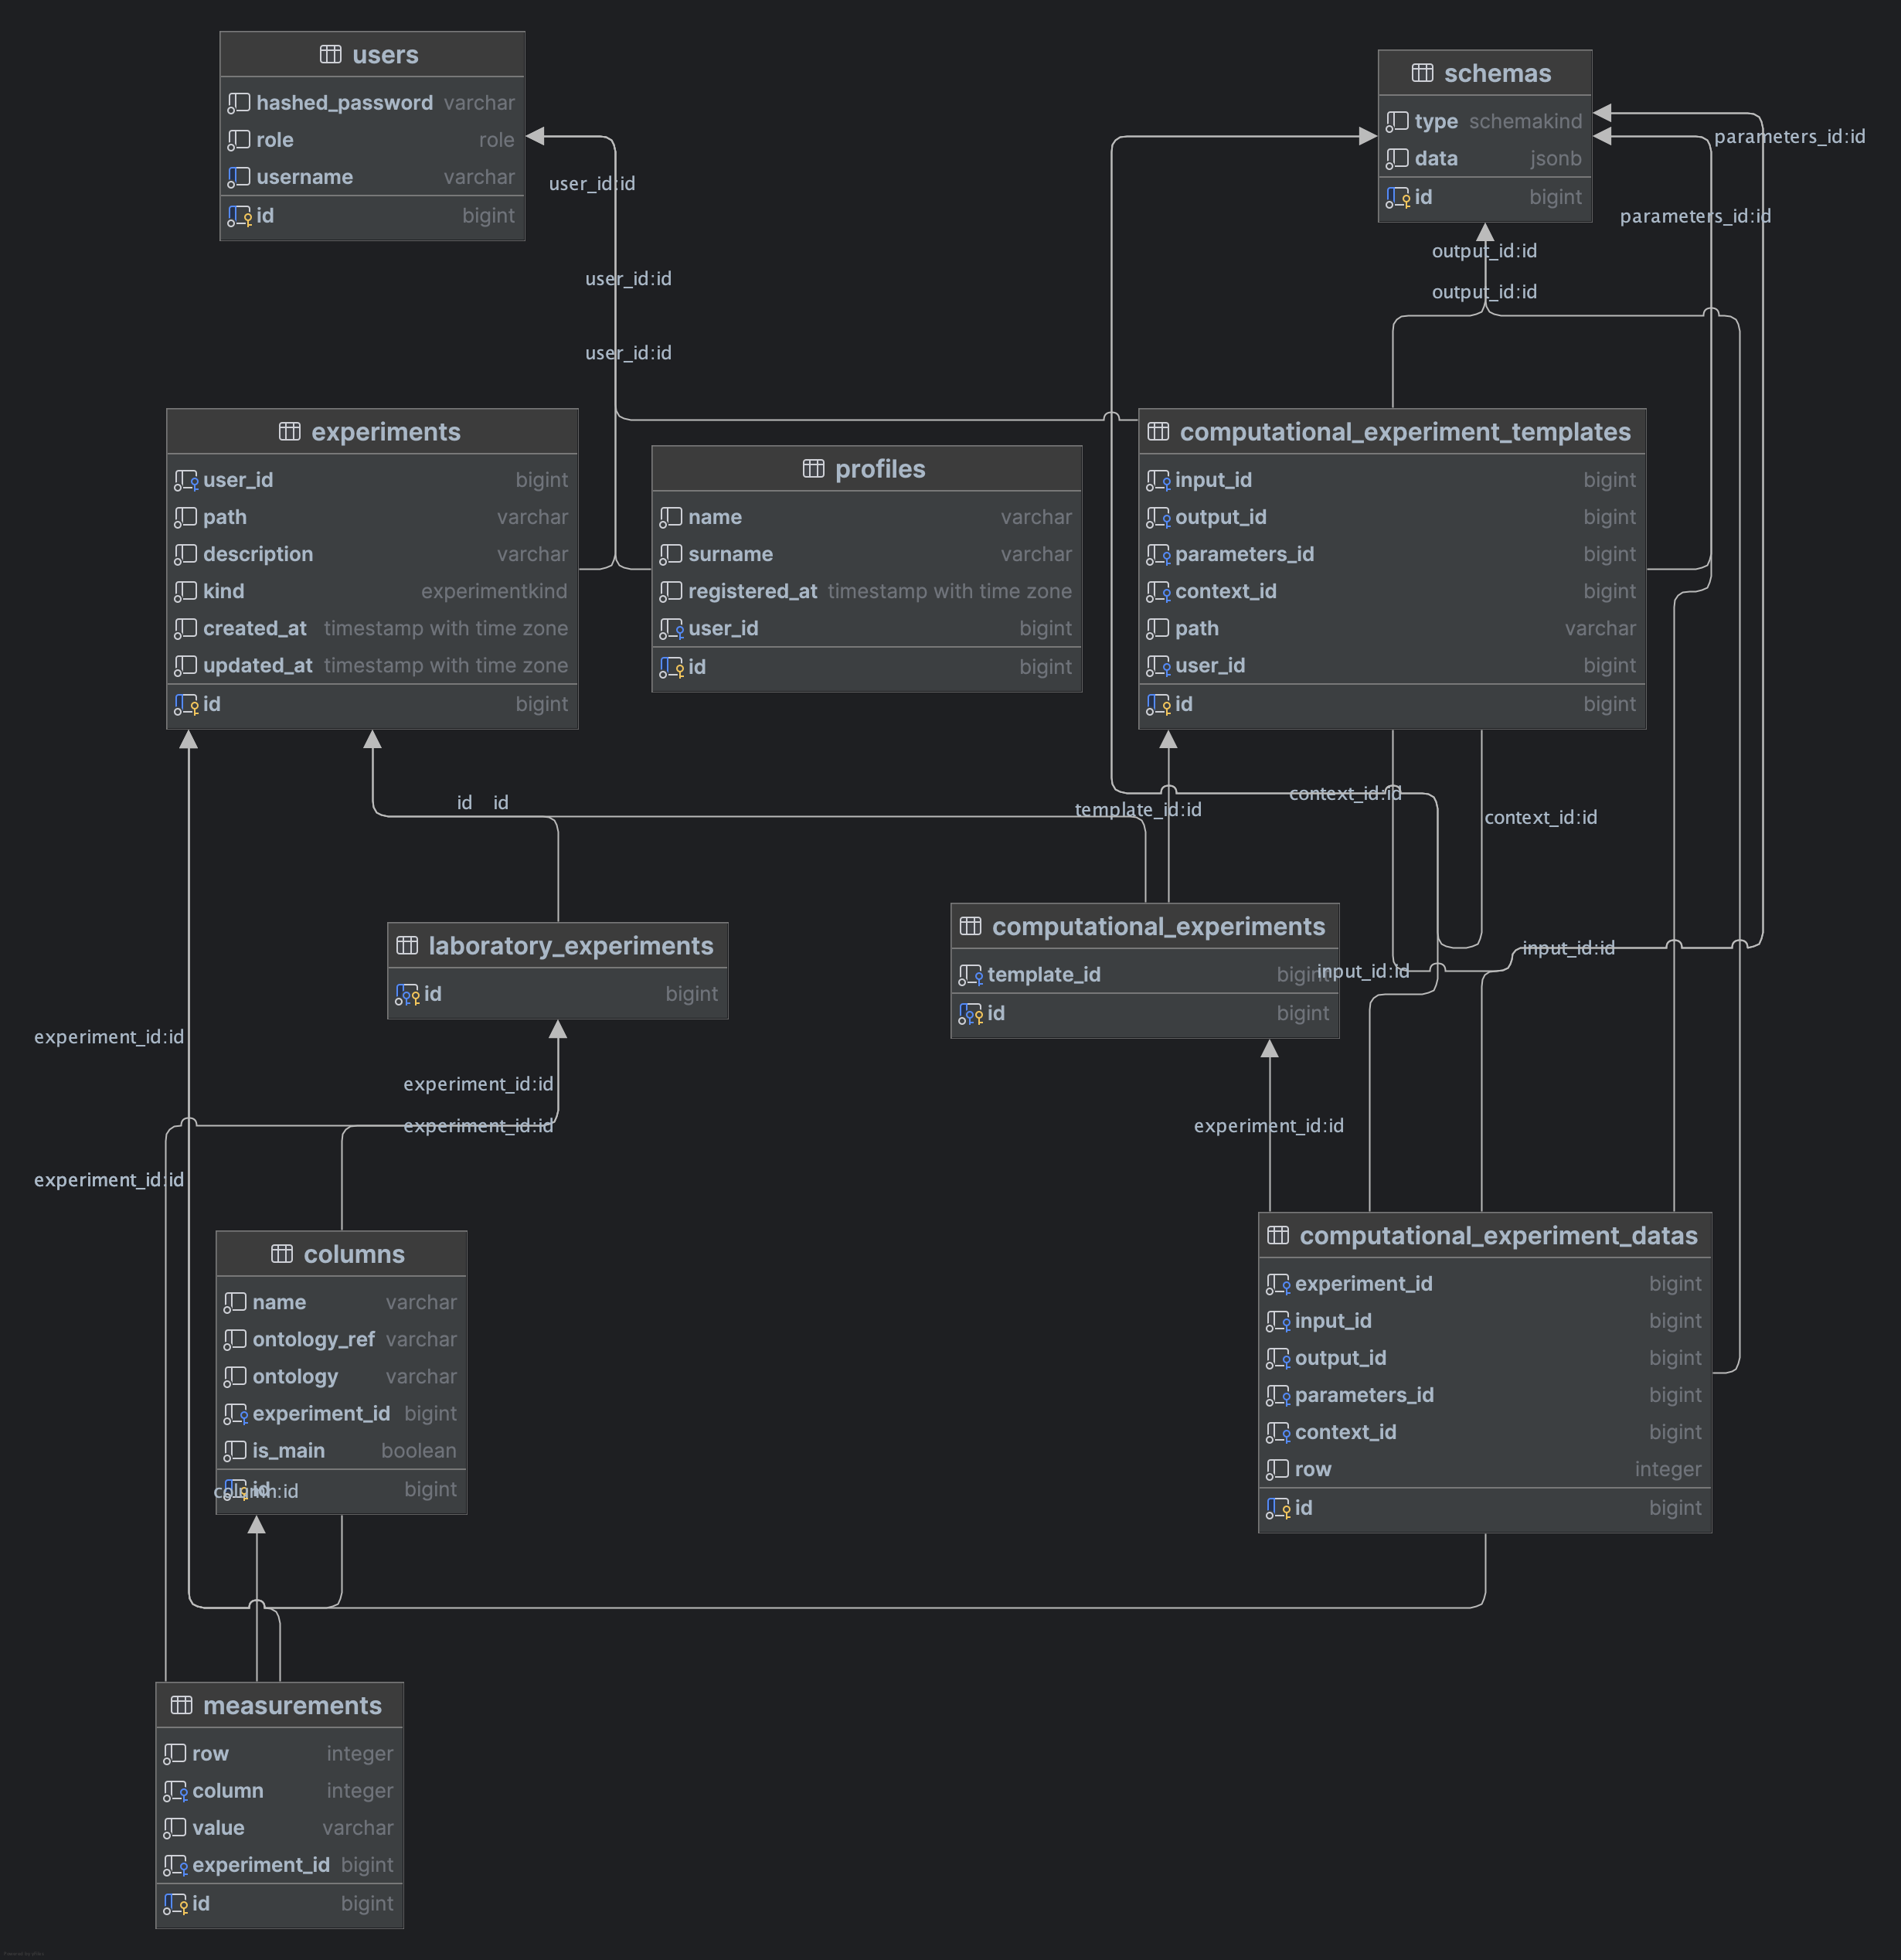
\includegraphics[width=\linewidth]{img/postgres_scheme.png}
\caption{Схема базы данных}
\label{pic:postgres_scheme}
\end{figure}
\vspace{0.5cm}

\subsubsection{ORM-модели}

Для работы с базой данных используется SQLAlchemy, обеспечивающая удобную работу с объектами и связями.
Модели представляют таблицы базы данных в виде классов, что позволяет писать гибкий и безопасный код.
ORM упрощает работу с базой, делает возможным автоматическое создание миграций для базы данных и сокращает количество SQL-запросов, оптимизируя их.

Основные сущности перечислены в~\ref{ORM models}.

\subsubsection{Управление миграциями}

Alembic используется для управления схемой базы данных, упрощая процесс обновления структуры данных без потери информации.
Среди возможностей этого инструмента особенно полезными можно назвать автоматическое создание миграций при изменении зарегистрированных моделей, возможность отката к предыдущим версиям схемы, и, как следствие, контроль изменений базы через версионирование.
Всё это позволяет плавно изменять схему базы, исключая конфликты данных.

\subsection{Интеграция с онтологиями}

\subsubsection{Способы привязки данных к онтологиям}

Каждый столбец таблицы измерений может быть связан с онтологией (рис.~\ref{pic:linked_to_ontology_column}), обеспечивая стандартную интерпретацию данных.
Связь осуществляется через указание для столбца псевдонима онтологии и элемента онтологии, зарегистрированной в приложении под этим псеводонимом.
Такое автоматизированное сопоставление данных снижает вероятность ошибок при интерпретации.

\begin{figure}[H]
\centering
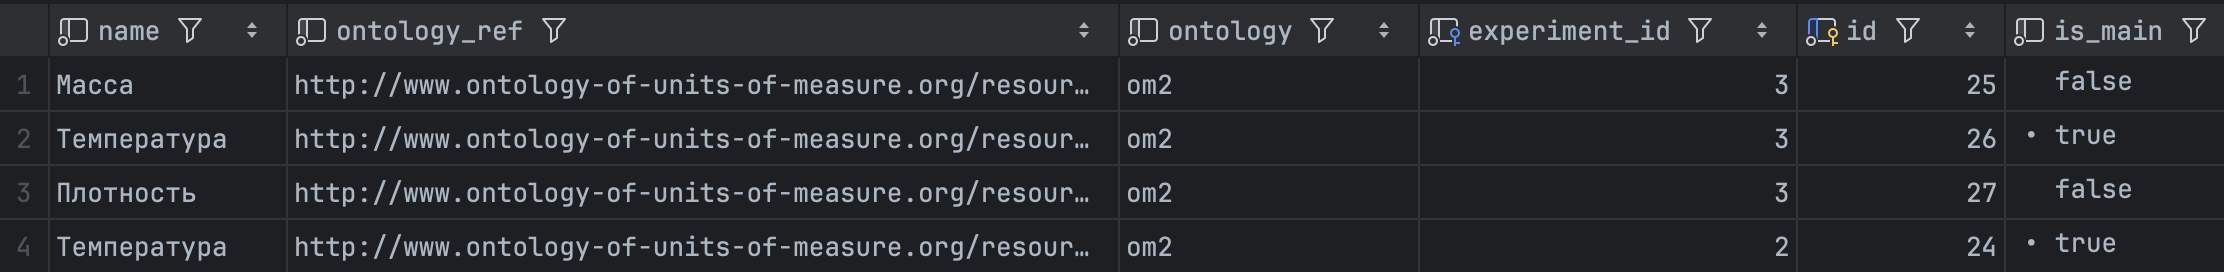
\includegraphics[width=\linewidth]{img/ontology_linking.png}
\caption{Столбец, привязанный к онтологии}
\label{pic:linked_to_ontology_column}
\end{figure}
\vspace{0.5cm}

\subsubsection{Поддерживаемые онтологии}

Приложение поддерживает две онтологии:
\begin{enumerate}
\item OM2 -- онтология физических величин и единиц измерения.
\item СhEBI -- онтология химических соединений.
\end{enumerate}

\subsubsection{Возможности расширения онтологической поддержки}

Система спроектирована таким образом, чтобы поддерживать подключение новых онтологий.
Добавление новых источников знаний требует лишь обновления базы данных, API и написания модуля со специфичными для онтологии запросами.

\subsection{Тестирование и отладка}

\subsubsection{Модульное тестирование серверной части}

Для тестирования серверной части используются unit-тесты (рис.~\ref{pic:backend_unit_tests}), написанные с использованием пакета pytest~\cite{Library:Pytest}, проверяющие корректность работы моделей, API и механизмов аутентификации.

\begin{figure}[H]
\centering
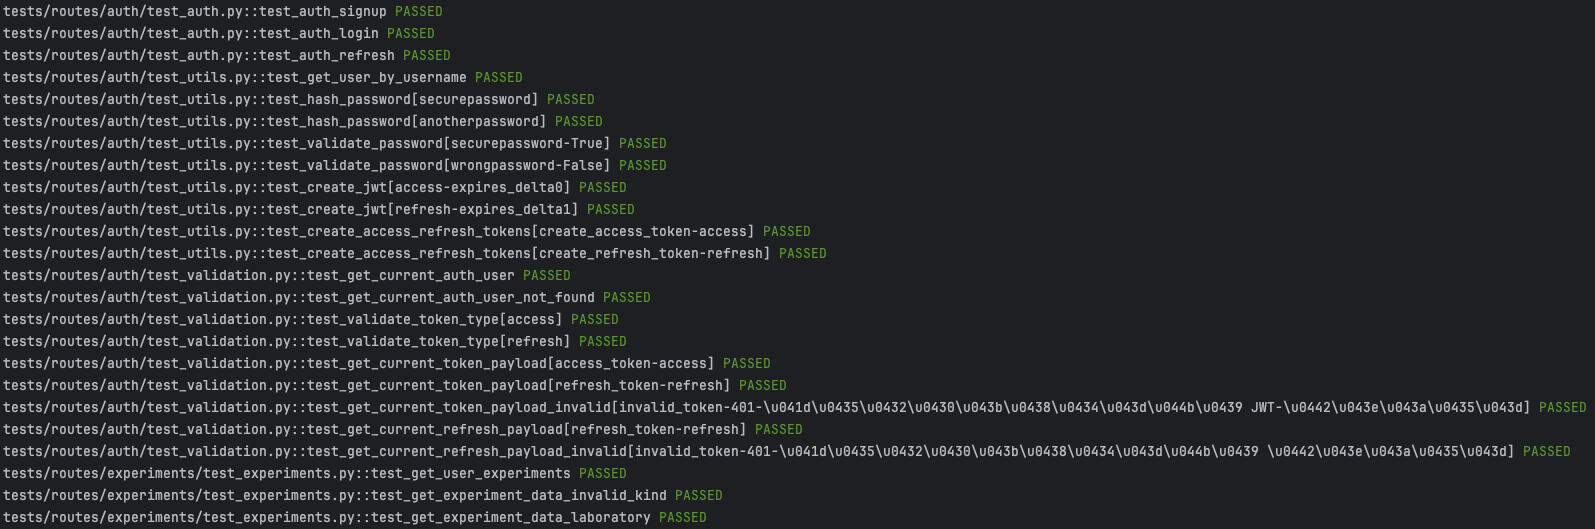
\includegraphics[width=\linewidth]{img/python_unit_tests.png}
\caption{Пример запуска unit-тестов серверной части}
\label{pic:backend_unit_tests}
\end{figure}
\vspace{0.5cm}

\subsubsection{Интеграционное тестирование API}

Для тестирования API применяется класс TestClient из FastAPI, который позволяет проверять работу маршрутов в изолированной среде.

% \subsubsection{Тестирование клиентской части}

% Фронтенд тестируется с помощью Cypress и Jest. Проверяются основные пользовательские сценарии: аутентификация, создание и редактирование экспериментов, работа с таблицами.

% \todo[inline]{Вставить пример теста интерфейса}

\subsection{Развёртывание и эксплуатация}

\subsubsection{Подготовка среды}

Приложение контейнеризовано с использованием Docker.
Все компоненты (серверная часть, клиентская часть, базы данных) запускаются через Docker Compose, обеспечивая предсказуемость окружения.
Это позволяет развернуть приложение на любом сервере без сложной настройки.
Также предусмотрены различные конфигурации Docker Compose, предназначенные специально для разработки, тестирования и продуктового окружения.

В продуктовом окружении приложение разворачивается с помощью Docker Compose, который управляет следующими сервисами:
\begin{enumerate}
\item backend -- контейнер с серверной частью.
\item frontend -- контейнер с обратным прокси-сервером для работы с клиентом.
\item db -- контейнер с PostgreSQL.
\item neo4j -- контейнер с Neo4j.
\end{enumerate}

\subsubsection{Настройка Nginx как обратного прокси}

Для маршрутизации запросов используется Nginx, который проксирует HTTP-запросы от фронтенда к бэкенду, а также управляет статическими файлами, что повышает общую производительность системы и отзывчивость для пользователя.

Основные настройки:
\begin{enumerate}
\item Проксирование API-запросов на бэкенд.
\item Кеширование статических файлов.
\end{enumerate}

\subsubsection{Запуск приложения}

Для запуска приложения необходимо предварительно заполнить конфигурационные файлы и воспользоваться системой контейнеризации Docker Compose.
Это обеспечивает воспроизводимость окружения и облегчает развёртывание как на локальной машине, так и на сервере.

\paragraph{Заполнение конфигурации} \mbox{}\\

Перед запуском требуется создать или отредактировать файлы переменных окружения для всех компонентов.
Для этого используются файлы \texttt{.env} в корне проекта и в директории \texttt{backend/config}.
В них указываются параметры подключения к базам данных, секретные ключи, настройки портов и прочие параметры.
Пример содержимого файла \texttt{.env} в листинге~\ref{lst:config_all}.
\begin{lstlisting}[frame=single, basicstyle=\footnotesize\ttfamily, label={lst:config_all}, caption={Заполнение конфигурационного файла всего приложения},captionpos=b, breaklines=true, breakatwhitespace=true, language=bash]
PG_USER=postgres
PG_PASSWORD=123
PG_DB=postgres

NEO4J_USER=neo4j
NEO4J_PASSWORD=123
\end{lstlisting}

Для запуска серверного приложения требуется создание в директории \texttt{backend/config} файла \texttt{config.stable.toml}, в котором нужно в формате TOML~\cite{Format:TOML} определить по крайней мере параметры \texttt{db.host}, \texttt{db.password}, \texttt{neo4j.host}, \texttt{neo4j.password}.
Также необходимо зарегистрировать онтологии по следующему принципу: секция \texttt{ontologies} представляет собой отображение, где ключ являются псевдонимом онтологий, которое затем может быть использовано в клиентском приложении, а значением – название метки, которая должна быть у каждого элемента онтологии.
Таким образом, если есть в секции \texttt{ontologies} пара, например, (OM2, om2UniqueLabel) приложение будет интерпретировать всякий результат запроса в Neo4j с меткой om2UniqueLabel как элемент онтологии OM2.

Пример содержимого файла \texttt{backend/config/config.stable.toml} в листинге~\ref{lst:config_backend}.
\begin{lstlisting}[frame=single, basicstyle=\footnotesize\ttfamily, label={lst:config_backend}, caption={Заполнение конфигурационного файла серверного приложения},captionpos=b, breaklines=true, breakatwhitespace=true]
[uvi]
host = ""
port = 0
workers = 0
timeout = 0
debug = false

[db]
port = 0
user = ""
database = ""
echo = false
echo_pool = false
pool_size = 0
max_overflow = 0
host = ""
password = ""

[neo4j]
port = 0
user = ""
db = ""
host = ""
password = ""

[jwt]
algorithm = ""
access_token_expire_minutes = 0
private_key_path = ""
public_key_path = ""
refresh_token_expire_minutes = 0

[ontologies]
OM2 = '__OntologyOM2__'
ChEBI = '__OntologyChEBI__'
\end{lstlisting}

\paragraph{Запуск с помощью Docker Compose} \mbox{}\\

После настройки переменных окружения приложение запускается одной командой: \texttt{docker-compose up --build}.
Эта команда соберёт и запустит все необходимые сервисы: серверную часть, клиентскую часть, базы данных PostgreSQL и Neo4j, а также Nginx для проксирования запросов.

Для запуска в фоновом режиме можно использовать флаг \texttt{-d}: \texttt{docker-compose up --build -d}

\paragraph{Дополнительные команды} \mbox{}\\

Для управления жизненным циклом приложения используются стандартные команды Docker Compose:
\begin{itemize}
\item Остановить сервисы: \texttt{docker-compose down}
\item Перезапустить сервисы: \texttt{docker-compose restart}
\item Просмотреть логи: \texttt{docker-compose logs -f}
\end{itemize}

\paragraph{Доступ к приложению} \mbox{}\\

После успешного запуска приложение становится доступно по адресу, указанному в настройках Nginx (по умолчанию \texttt{http://localhost/}).
Все компоненты приложения взаимодействуют друг с другом через внутреннюю сеть Docker Compose.

\anonsubsection{Выводы по главе}

В данной главе рассмотрена программная реализация веб-приложения, включая серверную и клиентскую части, работу с базой данных, интеграцию с онтологиями, тестирование и развёртывание. Архитектура приложения построена по клиент-серверной модели, обеспечивая высокую производительность и удобство работы с данными. Использование ORM упростило взаимодействие с базой данных, а поддержка онтологий позволила связывать экспериментальные данные с формализованными научными сущностями. Гибкое управление состоянием во фронтенде и система тестирования способствуют надёжности работы интерфейса и API. Развёртывание через контейнеризацию обеспечивает переносимость, а механизмы аутентификации и защиты данных гарантируют безопасность. В результате создана масштабируемая и расширяемая система для управления лабораторными и вычислительными экспериментами, адаптируемая к новым требованиям.

    \anonsection{Заключение}

В данной работе была рассмотрена проблема управления данными лабораторных и вычислительных экспериментов и предложено её решение в виде веб-приложения, обеспечивающего удобную работу с экспериментальными данными и их привязку к онтологиям.
Был проведён анализ предметной области, который показал, что существующие решения не позволяют эффективно стандартизировать данные и автоматически проверять корректность единиц измерения.
Разработка нового инструмента была направлена на устранение этих недостатков за счёт интеграции онтологий, структурированного хранения данных и удобного интерфейса для работы исследователей.

В процессе проектирования была определена архитектура системы, основанная на клиент-серверной модели.
Проработаны пользовательские сценарии, продумана структура базы данных и реализованы механизмы взаимодействия между компонентами системы.
В качестве ключевых требований были выделены поддержка онтологий, удобство работы с экспериментами и возможность гибкой настройки системы.
Разработанное приложение позволяет пользователям фиксировать и редактировать данные, организовывать эксперименты, привязывать измерения к онтологическим сущностям, а также получать удобный доступ к структурированной информации.

В ходе реализации была создана серверная часть, обеспечивающая надёжное хранение данных, обработку API-запросов и механизмы аутентификации.
Клиентская часть разработана с учётом удобства использования, что позволяет исследователям легко управлять экспериментами и их параметрами.
Интеграция с онтологиями позволяет стандартизировать данные, обеспечивая их корректную интерпретацию и автоматическое сопоставление единиц измерения.
Проведённое тестирование подтвердило работоспособность системы, а контейнеризация и автоматизация развертывания обеспечили удобство эксплуатации.

Перспективы дальнейшего развития приложения связаны с добавлением поддержки новых типов экспериментов, расширением возможностей по импорту и экспорту данных в различные форматы, а также интеграцией с внешними базами знаний.
Внедрение инструментов для визуализации экспериментальных данных и статистического анализа позволит повысить удобство работы пользователей и сделать приложение более универсальным для различных научных областей.

\newpage
\printbibliography[title=Список источников, heading=bibintoc]
\newpage

\addition{Техническое задание}{TZ}
Представлено отдельным документом <<Техническое задание. Веб-приложение для ведения лабораторных и вычислительных экспериментов с поддержкой онтологий\unskip>>.

\addition{Руководство оператора}{RO}
Представлено отдельным документом <<Руководство оператора. Веб-приложение для ведения лабораторных и вычислительных экспериментов с поддержкой онтологий\unskip>>.

\addition{Программа и методика испытаний}{PMI}
Представлено отдельным документом <<Программа и методика испытаний. Веб-приложение для ведения лабораторных и вычислительных экспериментов с поддержкой онтологий\unskip>>.

\addition{Текст программы}{TP}
Представлено отдельным документом <<Текст программы. Веб-приложение для ведения лабораторных и вычислительных экспериментов с поддержкой онтологий\unskip>>.

\end{document}